% Master Thesis Report
% Created by: Claes Arvidson and Emelie Karlsson 
% Linköping University Spring 2016
% First version: 2016-01-27

\documentclass[a4paper, 10pt, twoside, openright]{book}
\pagestyle{headings}

% some of the packages used are
\usepackage[round, authoryear]{natbib}
\bibliographystyle{unsrtnat}
\usepackage{xcolor, colortbl}
\usepackage{tabularx}
\usepackage{latexsym}
\usepackage{eepic}
\usepackage{makeidx}
\usepackage{booktabs}
\usepackage{graphicx}
\usepackage[utf8]{inputenc}  %för ä ö å ?
\usepackage[english]{babel}
%\usepackage{times}
\usepackage{amssymb}
%\usepackage{fancybox} 
%\usepackage{textcomp}
\usepackage{float}
%\usepackage{amsmath}
\usepackage{mathtools}
\usepackage{multirow}
\usepackage{footnote}
%\makesavenoteenv{tabular}
%\makesavenoteenv{table}
\usepackage{tikz}
\usetikzlibrary{shapes,arrows}

% the fancy header/footer
% consult http://research.cmis.csiro.au/gjw/tex/docs/fancyhdr.pdf
% or some other fancy header documenatation for more info
\usepackage{fancyhdr}
\pagestyle{fancy}
\lfoot{\nouppercase{\rightmark}}
\rfoot{\nouppercase{\leftmark}}
\fancyfoot{} 
\fancyhead[LO]{\nouppercase{\small{\rightmark}}}
\fancyhead[RE]{\nouppercase{\small{\leftmark}}}
\fancyhead[LE,RO]{\small{\thepage}}
\fancyhead[C]{}
\renewcommand{\footrulewidth}{0pt}
\renewcommand{\headrulewidth}{0.2pt}
\fancypagestyle{plain}{ \fancyhf{}  
  \fancyfoot[RE,LO]{\nouppercase{\small{\putegotext}}}
  \fancyfoot[LE,RO]{\small{\thepage}}
  \renewcommand{\headrulewidth}{0pt}  \renewcommand{\footrulewidth}{0.2pt} }

\newcommand\mydots{\hbox to 1em{.\hss.\hss.}}
% ------------------------------------------------------------------------
% BEGINNING of abstract, author, examiner, etc
% here you must fill in your own text. Remember to respect the { and the }.
%
% the *-marked % in 
%                                   *
%      \newcommand{\putabstract}[0]{% 
%      some text}
%
% is made to avoid a blank space in the beginning of the abstract,
% author, date etc.
%
\newcommand{\putabstract}[0]{%
Here is where you can write your abstract. It may be very long, or it
may be very short, the reason you have an abstract is for people not
to be forced to read lots of crap.

But still, they will have to read your abstract. After all, the
abstract is what everyone reads\ldots}

\newcommand{\putkeywords}[0]{%
Keyword One, Chemostat, Another Key-Word, Key, Clé, Mot de cle,
Nyckelhål, XBOX, Dagens viktigaste nyckelord, and Keywords.}

\newcommand{\putthemonth}[0]{June }

\newcommand{\putshortdate}[0]{2016}

\newcommand{\putmydate}[0]{\putthemonth \putshortdate}

\newcommand{\putauthor}[0]{Claes Arvidson, Emelie Karlsson}

\newcommand{\putegotext}[0]{Arvidson, Karlsson, 2016.}

\newcommand{\puttitle}[0]{Work Distribution of a Heterogeneous Library Staff - A Personnel Task Scheduling Problem}

% some kind of administrator will give you this number
\newcommand{\putregnumber}[0]{LiTH - MAT - EX - - 04 / 04 - - SE}

\newcommand{\putexaminer}[0]{E. Rönnberg}

\newcommand{\putsupervisor}[0]{T. Larsson}

% for example Applied Mathematics
\newcommand{\putdepartment}[0]{Optimeringslära}

% send an email to ep.liu.se to make sure it is correct before you print
% this number is the one I had
\newcommand{\putmyurl}[0]{http://www.ep.liu.se/exjobb/mai/2004/tm/004/}

% Please do not change into University of Linköping or something, the
% international name of Liu is Linköpings Universitet
\newcommand{\putliu}[0]{Linköpings Universitet}

%Create the command \tab
\newcommand{\tab}[1]{\hspace{.2\textwidth}\rlap{#1}}
\newcommand{\itab}[1]{\hspace{0em}\rlap{#1}}
\DeclarePairedDelimiter\abs{\lvert}{\rvert}
\DeclarePairedDelimiter\norm{\lVert}{\rVert}
%
% END of abstract, author, examiner, etc
% ------------------------------------------------------------------------

\begin{document} 

\frontmatter
\raggedbottom
% some new commands I used, you won't need them I guess- just erase it
\newcommand{\ala}[0]{{\alpha}_{1}}
\newcommand{\alb}[0]{{\alpha}_{2}}
\newcommand{\nc}[0]{{N}_{C}}
\newcommand{\tCh}[0]{the Chemostat }
\newcommand{\Ch}[0]{Chemostat }
\newcommand{\ch}[0]{chemostat }
\newcommand{\MMk}[0]{Michaelis-Menten kinetics }
\newcommand{\KI}[0]{{K}_{I} }
\newcommand{\KN}[0]{{K}_{N} }
\newcommand{\mmu}[0]{{\mu}_{max} }
\newcommand{\KMAX}[0]{\mmu}
\newcommand{\AAA}[0]{\mathbf{A} }
% stop erasing here

%\usepackage[first=0,last=9]{lcg}
%\newcommand{\ra}{\rand0.\arabic{rand}}

% Colors
\newcommand{\enc}[0]{utf8}
\definecolor{bluegray}{rgb}{0.4, 0.6, 0.8}
\definecolor{darkcyan}{rgb}{0.0, 0.55, 0.55}
\definecolor{corn}{rgb}{0.98, 0.93, 0.36}
\definecolor{coralred}{rgb}{1.0, 0.25, 0.25}
\definecolor{Gray}{gray}{0.85}
\definecolor{Darkgray}{gray}{0.9}
\definecolor{maroon}{cmyk}{0,0.87,0.68,0.32}
\newcommand{\colcell}{\cellcolor{Gray}}
\newcommand{\colcelltwo}{\cellcolor{corn}}
\newcommand{\colcellthree}{\cellcolor{darkcyan}}
\newcolumntype{g}{>{\columncolor{corn}}c}

% Special cells
\newcommand{\specialcell}[2][c]{%
  \begin{tabular}[#1]{@{}l@{}}#2\end{tabular}}
\newcommand{\specialcelltwo}[2][c]{%
   \begin{tabular}[#1]{@{}l@{}l@{}}#2\end{tabular}}
\newcolumntype{L}[1]{>{\raggedright\let\newline\\\arraybackslash\hspace{0pt}}m{#1}}
\newcolumntype{C}[1]{>{\centering\let\newline\\\arraybackslash\hspace{0pt}}m{#1}}
\newcolumntype{R}[1]{>{\raggedleft\let\newline\\\arraybackslash\hspace{0pt}}m{#1}}


% don't mind these
\title{\puttitle}
\author{\putauthor}

% this command makes the first page, and the second page, handle with care
% You really don't have to change anything here I guess.
\renewcommand{\maketitle}{%
              \newpage%
              \pagestyle{empty}
              \null%
              \hfil\hspace*{-3mm}
              \begin{minipage}{150mm}
                \center 
                {\Large{Master thesis}} \\\vspace*{4mm}
                {\vbox to 22mm{\vfil\Large\textbf{\puttitle}}}
                \vspace*{5mm}
                 {\Large{\putauthor}}       \\ \vspace*{4mm}
                  \putregnumber\\
                \end{minipage}\hfil
              \clearpage%\hspace*{0mm}\thispagestyle{empty}
              \clearpage%\thispagestyle{empty}
              \null%
              \hfil\hspace*{-3mm}
              \begin{minipage}{150mm}
                \center
                {\vbox to 48mm{\vfil\Large\textbf{\puttitle}}}
                \vspace*{5mm}
                  \putdepartment, \putliu \\ \vspace*{4mm}
                  \textbf{\putauthor}       \\ \vspace*{4mm}
                  \putregnumber
                  \vspace*{100mm}\\
                \flushleft
                
                Exam work:\hspace*{3pt}
                \begin{minipage}[t]{70mm}
% but you might want to change this 30
                  \textbf{30 hp}
                \end{minipage} \\ \vspace*{4mm}
                
                Level:\hspace*{3pt}
                \begin{minipage}[t]{70mm}
% and you might want to change this A 
                  \textbf{A} 
                \end{minipage} \\ \vspace*{4mm}
                
                Supervisor:\hspace*{3pt}
                \begin{minipage}[t]{120mm}
                  \textbf{\putsupervisor}, \\\putdepartment, \putliu
                \end{minipage} \\ \vspace*{4mm}
                
                Examiner:\hspace*{3pt}
                \begin{minipage}[t]{120mm}
                  \textbf{\putexaminer}, \\\putdepartment, \putliu
                \end{minipage} \\ \vspace*{4mm}
                
                Linköping:
                \begin{minipage}[t]{70mm}
                  \textbf{\putmydate}
                \end{minipage} \\ \vspace*{4mm}
              \end{minipage} \\ \hfill
}

% now the \maketitle command is changed and we use the new one
\maketitle

% I'm not sure this phantom is needed, but I leave to make sure
% a phantom leaves empty space corresponding to the size of what is in it.
\phantom{crap}
\thispagestyle{empty}
\pagestyle{empty}

\setlength{\unitlength}{1mm}


\setlength{\unitlength}{1pt}

% now turn on fancy headers
\pagestyle{fancy}

% ..................chapter ...............................................
\chapter*{Abstract\index{Abstract}}
% your abstract
\putabstract

% enters keywords
\begin{description}
\item[Keywords:]{%
\putkeywords
}
\item[URL for electronic version: ]{\hfill%\quad\\%
%\phantom{\qquad} http://urn.kb.se/resolve?urn=urn:nbn:se:liu:diva-77777\\
%where 77777 should be replacd by an appropriate number.
\begin{center}
http://urn.kb.se/resolve?urn=urn:nbn:se:liu:diva-77777
\end{center}
%where 77777 should be replaced by an appropriate number.
}
\end{description}


% here or on the next page you put an abstract in swedish
%\section*{Abstract in Swedish: Sammanfattning}
%Det finns många typer av bioreaktorer som tillämpas\ldots

\chapter*{Acknowledgements\index{Acknowledgements}}

I would like to thank my supervisor, I would like to thank my
supervisor, I would like to thank my supervisor, I would like to thank my supervisor\ldots

I also have to thank, I would like to thank my supervisor, I would
like to thank my supervisor, I would like to thank my supervisor, I
would like to thank my supervisor\ldots

My opponent NN also deserves my thanks, I would like to thank my
supervisor, I would like to thank my supervisor, I would like to thank my supervisor\ldots





% optional I guess
\chapter*{Nomenclature\index{Nomenclature}}

Most of the reoccurring definitions, symbols and abbreviations are described here.

%----------------NEW_SECTION--------------------------------------------------
\section*{Definitions\index{Definitions}}
\begin{tabular}{lp{10cm}}

Heuristic & An algorithm designed to find sufficiently good, but not necessarily optimal solutions. \\
Fetch list & The library task of collecting books from shelves that are to be delivered elsewhere. \\
Library on wheels & The library task of driving the bus with books to remote areas of town. \\
%Rostering & \\
%Matheuristic & Text\\
\end{tabular}

\section*{Symbols\index{Symbols}}

%\begin{tabular}{ll}
%$Y_0$      & The amount of the variable $Y$ inserted into a system.\\
%$\hat Y$& The unit-dimension of the variable $Y$, for example $\hat t=1s$ .\\
%$\bar Y_i$ & A steady state (number $i$) value of Y.\\
%\phantom{a}& \phantom{b} \\
%$K_i$ & Constants used in kinetic expressions, for example $K_I$.\\
%\phantom{a}& \phantom{b} \\
%$\AAA$     & The system matrix. \\
%\end{tabular}

\section*{Abbreviations\index{Abbreviations}}

\begin{tabular}{ll}
Exp		& Service counter(sv. expeditionsdisken) \\
Info	& Information counter (sv. informationsdisken)\\
PL		& Fetch list (sv. plocklistan)\\
BokB    & Library on wheels (sv. bokbussen)\\
HB      & Hageby library \\
\end{tabular}


\tableofcontents 
\begin{samepage}
\listoffigures
\let\clearpage\relax
\listoftables
\end{samepage}


\mainmatter

%##########################################################
% -------------------CHAPTERS -----------------------------
%##########################################################

\chapter{Introduction}\label{chap:intro}

\inputencoding{\enc}
% Introduction to Master Thesis

\section{Background}


At a library, staff absence can cause problems and result in a shortage of staff with a special competence. If a worker is unavailable a certain day due to a meeting or illness it would require a stand-in to fill the vacancy. Therefore, it is of great interest to create schedules with as many skilled stand-ins as possible to overcome such disturbances, when they occur. Furthermore, the library personnel have certain demands and preferences as to how a satisfactory working schedule should be. For instance, it is neither preferable to work more than one evening per week nor work more weekends than required. 

The problem addressed in this thesis work concerns the library staff at the Central Library of Norrköping. The library has more than 40 employees and the culturally important building from the 1950's is known to all inhabitants of Norrköping. The library is open weekdays between 08:00 and 20:00 and during weekends between 11:00 and 16:00. The generous opening times also creates a challenge for the library as it requires a large pool of well coordinated personnel to keep it running. In addition, the library also provides its services to one other smaller library. This creates a challenge for the library schedulers.

\section{Problem description}

In this section, the most important features of the worker scheduling problem studied in this thesis work will be explained.  

\subsection{Description of the daily tasks at the library} \label{section:library_tasks}
The most important activity at a library is the activity directed towards the public. This includes book loan services as well as providing customers with helpful information about the resources at the disposal of the library. These activities are referred to as "outer tasks". In addition, the book collection must be maintained, the returned books must be sorted and put back to the shelves, the web page must be updated and so on. Such work is often referred to as "inner work" and this non-public work is an equally important part of the everyday activities at the library. 

Three main outer task types can be identified at the library of Norrköping, working in the service counter (sv. expiditionsdisken), working in the information counter (sv. informationsdiken)  and assembling books which are to be sent to other libraries according to the "fetch list" (sv. plocklista). The fetch list is a task type for which the worker is scheduled during a whole day, while the other task types have two to five hour shifts. The outer tasks can be performed by either librarians or both, as described in Table \ref{tab:Outer_Tasks}.

\begin{table}[h]
\centering
\caption{Outer tasks can be performed exclusively by librarians or by both librarians and assistants.}
\label{tab:Outer_Tasks}
\begin{tabularx}{\textwidth}{|l|l|X|}
\hline
%-------------------------------------------------------------------
\textbf{Task} & \textbf{Description} & \textbf{Qualification}\\ \hline 
%------------------------------------------------------------------- 
\specialcell[t]{Service counter \\ (Exp)}  & \specialcell[t]{Administring loans, library cards\\ and the loaning machine} & \specialcell[t]{Librarian or \\  assistant} 
%\begin{tabular}[x]{@{}c@{}}\\\end{tabular}  
\\ \hline
%-------------------------------------------------------------------
\specialcell[t]{Information counter \\ (Info)} & \specialcell[t]{Handling questions \\about the library's resources.} & Librarian
\\ \hline 
%-------------------------------------------------------------------
\specialcell[t]{Fetch list \\(PL)} & \specialcell[t]{Fetching books that are to be \\sent to other libraries.} & \specialcell[t]{Librarian  or \\  assistant}
\\ \hline 
%-------------------------------------------------------------------
\specialcell[t]{Hageby \\(HB)} & \specialcell[t]{Handling librarian tasks at the filial \\ Hageby during weekends.} & Librarian
\\ \hline 
%-------------------------------------------------------------------
\specialcell[t]{Library on Wheels \\(BokB)} & \specialcell[t]{Driving the Library on Wheels \\ to different areas of town.} & Librarian
\\ \hline 
%-------------------------------------------------------------------
\end{tabularx}
\end{table} 

Since the number of visitors at the library varies throughout the day and also during different days of the week, so does the demand for personnel for the three tasks. The demand of personnel for the different task types is illustrated in Table \ref{tab:Outer_Task_Demand}, according to figures given by the library. 



\begin{table}[h]
\centering
\caption{Demand of staff for the three daily tasks.}
\label{tab:Outer_Task_Demand}
\begin{tabularx}{\textwidth}{|X|l|l|l|l|X|}
\hline
%-------------------------------------------------------------------
\textbf{Day} & \textbf{Time} & \textbf{Exp demand} & \textbf{Info demand} & \textbf{PL demand\footnote{The Fetch list is a whole day task covering three consecutive shifts which must be performed by the same worker.}}
\\ \hline 
%------------------------------------------------------------------- 
Mon-Fri & 08:00-10:00 & 2 & 2 & 1
\\ \hline 
%------------------------------------------------------------------- 
Mon-Fri & 10:00-13:00 & 3 & 3 & 1
\\ \hline 
%-------------------------------------------------------------------
Mon-Fri & 13:00-16:00  & 3 & 3 & 1
\\ \hline 
%-------------------------------------------------------------------
Mon-Fri & 16:00-20:00 & 3 & 3 & -
\\ \hline 
%-------------------------------------------------------------------
Sat & 11:00-16:00  & 3 & 3 & -
\\ \hline 
%------------------------------------------------------------------- 
Sun & 11:00-16:00  & 3 & 3 & -
\\ \hline 
%------------------------------------------------------------------- 
\end{tabularx}

\end{table} 

As in the case with most libraries, the Central Library of Norrköping also has responsibilities that fall outside of its normal daily activities. One such responsibility is the running of a smaller library filial in Hageby, situated in a suburban area of Norrköping, during weekends. It is decided that only librarians are qualified for this task, as it implies some tasks that need certain knowledge.

Table \ref{tab:Hageby_Demand} shows the demand of staff at Hageby. Worth noting is that it is the same person working at Hageby a weekend due to a couple of reasons. Since a worker is supposed to work both Saturday and Sunday when due for a weekend, it is more desirable to let the worker focus on the same task both days. Furthermore, since Hageby is located in a suburban, some travel distance is required to reach it. This is compensated by letting the worker at Hageby be free from work Friday evening, which otherwise is included in the weekend work. 

\begin{table}[H]
\centering
\caption{Demand of staff at Hageby}
\label{tab:Hageby_Demand}
\begin{tabularx}{0.5\textwidth}{|l|l|X|}
\hline
%-------------------------------------------------------------------
\textbf{Day} & \textbf{Time} & \textbf{HB demand}
\\ \hline 
%%------------------------------------------------------------------- 
Sat & 11:00-16:00  & 1 
\\ \hline 
%%-------------------------------------------------------------------
Sun & 11:00-16:00  & 1 
\\ \hline 
\end{tabularx}
\end{table} 

Similarly, only a handful librarians are qualified for the task known as the "Library on Wheels" (sv. Bokbussen), which is a library bus that provides citizens in remoter areas of the city with books and other library services. The Library on Wheels only operates a few times a week and the schedule differs between odd and even weeks.

\begin{table}[!h]
\centering
\caption{Demand of staff Library on Wheels}
\label{tab:LOW_Demand}
\begin{tabularx}{0.80\textwidth}{|l|X|X|X|X|X|}
\hline
%%-------------------------------------------------------------------
 \textbf{Odd Week} & \textbf{Mon} & \textbf{Tue} & \textbf{Wed} & \textbf{Thu} & \textbf{Fri} 
 \\ \hline 
%%------------------------------------------------------------------- 
\rowcolor{Gray} 
08:00-10:00 & 1 & 0 & 1 & 1 & 1 
\\ \hline 
%%------------------------------------------------------------------- 
\rowcolor{Gray} 
16:00-20:00 & 1 & 0 & 1 & 1 & 0 
\\ \hline 
%%-------------------------------------------------------------------
 \textbf{Even Week} & \textbf{Mon} & \textbf{Tue} & \textbf{Wed} & \textbf{Thu} & \textbf{Fri} 
 \\ \hline 
%%------------------------------------------------------------------- 
\rowcolor{Gray} 
08:00-10:00 & 1 & 0 & 1 & 1 & 0 
\\ \hline 
%%------------------------------------------------------------------- 
\rowcolor{Gray} 
16:00-20:00 & 0 & 0 & 1 & 1 & 0 
\\ \hline 
\end{tabularx}
\end{table}

Apart from the outer work described above, there is also inner work at the library which sometimes need to be scheduled. One such type of inner work is meetings, as it concerns a large number of staff. Both library meetings, scheduled for the whole work force, and department meetings, scheduled only a subset of workers, exist. The library meetings are fixed in time and take place every fifth weeks on Monday mornings 8:15-10:00 while the department meetings are more flexible and take place every fifth week. For this, all department members must be available. Only three departments have scheduled meetings: the child department, the adult department and the media department.

\subsection{Personnel attributes}

At a library, the main group of workers are librarians and assistants (also janitors, cleaners, security guards etc.). The librarians make sure the library's resource collection is up to date, that the visitors find what they're looking for and perform a larger number of inner tasks. Assistants can perform most of theses tasks, while others require librarian competence.

The Central Library of Norrköping currently has 39 workers, 23 of which are librarians and 16 of which are assistants. All staff have different availability for performing tasks, depending on their working hours and the amount of inner work they are in charge of. In the standard case, each worker is assigned one evening per week and once per five weeks he/she is assigned to work during the weekend. The following week after a weekend is compensated by two free days, placed according to the wishes of the worker.

Let us consider a sample worker who is qualified for the same tasks as a librarian, works full time and is also assigned to work on Wednesday evenings. The worker is also assigned to work weekend on the fourth week and has chosen to take out its days off on Thursdays and Fridays on week five. The workers availability is thus illustrated in table \ref{tab:Bob_avail}. The schedule repeats itself after five weeks and illustrates only the availability for tasks but says nothing about whether the worker has been assigned any tasks or not.

All workers have a five week schedule in the same manner as the sample worker. However, in order to meet the weekend demands illustrated by Tables \ref{tab:Outer_Task_Demand}, \ref{tab:LOW_Demand} and \ref{tab:Hageby_Demand}, it is evident that not all workers can be assigned for weekend work at week 4. Instead, a worker's schedule should be seen as a \textit{relative schedule}, which can be shifted by whole weeks. We refer to this as the \textit{week rotation}.

The relative schedule is relative to the \textit{overall schedule} for the library. If the sample worker for example has week rotation 1, this means the weekend week in his relative schedule would be shifted to week 1 in the overall schedule. In Table \ref{tab:Bob_avail}, the weekend rotation is 4.



\begin{table}[!h]
\centering
\caption{Availability schedule for a sample worker. Yellow signifies that the worker is available. In parenthesis, the weekend shift. The week rotation is 4}
\label{tab:Bob_avail}
\begin{tabularx}{\textwidth}{|X|l|l|l|l|l|l|l|X|}
\hline
%-------------------------------------------------------------------
\textbf{Week 1}& \colcell \textbf{Mon} & \colcell \textbf{Tue} & \colcell \textbf{Wed} & \colcell \textbf{Thu} & \colcell \textbf{Fri} & \colcell \textbf{Sat} & \colcell \textbf{Sun}
\\ \hline 
%%------------------------------------------------------------------- 
%\rowcolor{Gray} 
\colcell 08:00-10:00 (11:00-16:00) & \colcelltwo & \colcelltwo & \colcelltwo & \colcelltwo & \colcelltwo & & 
\\ \hline 
%%-------------------------------------------------------------------
%\rowcolor{Gray} 
\colcell 10:00-13:00 & \colcelltwo & \colcelltwo & \colcelltwo & \colcelltwo & \colcelltwo &   & 
\\ \hline 
%%-------------------------------------------------------------------
%\rowcolor{Gray} 
\colcell 13:00-16:00 & \colcelltwo & \colcelltwo & \colcelltwo & \colcelltwo & \colcelltwo & &
\\ \hline 
%%-------------------------------------------------------------------
%\rowcolor{Gray} 
\colcell 16:00-20:00 & & & \colcelltwo & & & &
\\ \hline 
%%-------------------------------------------------------------------
\end{tabularx}
\begin{tabularx}{\textwidth}{|X|l|l|l|l|l|l|l|X|}
\hline
%-------------------------------------------------------------------
\textbf{Week 2}& \colcell \textbf{Mon} & \colcell \textbf{Tue} & \colcell \textbf{Wed} & \colcell \textbf{Thu} & \colcell \textbf{Fri} & \colcell \textbf{Sat} & \colcell \textbf{Sun}
\\ \hline 
%%------------------------------------------------------------------- 
%\rowcolor{Gray} 
\colcell 08:00-10:00 (11:00-16:00) & \colcelltwo & \colcelltwo & \colcelltwo & \colcelltwo & \colcelltwo & & 
\\ \hline 
%%-------------------------------------------------------------------
%\rowcolor{Gray} 
\colcell 10:00-13:00 & \colcelltwo & \colcelltwo & \colcelltwo & \colcelltwo & \colcelltwo &   & 
\\ \hline 
%%-------------------------------------------------------------------
%\rowcolor{Gray} 
\colcell 13:00-16:00 & \colcelltwo & \colcelltwo & \colcelltwo & \colcelltwo & \colcelltwo & &
\\ \hline 
%%-------------------------------------------------------------------
%\rowcolor{Gray} 
\colcell 16:00-20:00 & & & \colcelltwo & & & &
\\ \hline 
%%-------------------------------------------------------------------
\end{tabularx}
\begin{tabularx}{\textwidth}{|X|l|l|l|l|l|l|l|X|}
\hline
%-------------------------------------------------------------------
\textbf{Week 3}& \colcell \textbf{Mon} & \colcell \textbf{Tue} & \colcell \textbf{Wed} & \colcell \textbf{Thu} & \colcell \textbf{Fri} & \colcell \textbf{Sat} & \colcell \textbf{Sun}
\\ \hline 
%%------------------------------------------------------------------- 
%\rowcolor{Gray} 
\colcell 08:00-10:00 (11:00-16:00) & \colcelltwo & \colcelltwo & \colcelltwo & \colcelltwo & \colcelltwo & & 
\\ \hline 
%%-------------------------------------------------------------------
%\rowcolor{Gray} 
\colcell 10:00-13:00 & \colcelltwo & \colcelltwo & \colcelltwo & \colcelltwo & \colcelltwo &   & 
\\ \hline 
%%-------------------------------------------------------------------
%\rowcolor{Gray} 
\colcell 13:00-16:00 & \colcelltwo & \colcelltwo & \colcelltwo & \colcelltwo & \colcelltwo & &
\\ \hline 
%%-------------------------------------------------------------------
%\rowcolor{Gray} 
\colcell 16:00-20:00 & & & \colcelltwo & & & &
\\ \hline 
%%-------------------------------------------------------------------
\end{tabularx}
\begin{tabularx}{\textwidth}{|X|l|l|l|l|l|l|l|X|}
\hline
%-------------------------------------------------------------------
\textbf{Week 4}& \colcell \textbf{Mon} & \colcell \textbf{Tue} & \colcell \textbf{Wed} & \colcell \textbf{Thu} & \colcell \textbf{Fri} & \colcell \textbf{Sat} & \colcell \textbf{Sun}
\\ \hline 
%%------------------------------------------------------------------- 
%\rowcolor{Gray} 
\colcell 08:00-10:00 (11:00-16:00) & \colcelltwo & \colcelltwo & \colcelltwo & \colcelltwo & \colcelltwo & \colcelltwo & \colcelltwo
\\ \hline 
%%-------------------------------------------------------------------
%\rowcolor{Gray} 
\colcell 10:00-13:00 & \colcelltwo & \colcelltwo & \colcelltwo & \colcelltwo & \colcelltwo &   & 
\\ \hline 
%%-------------------------------------------------------------------
%\rowcolor{Gray} 
\colcell 13:00-16:00 & \colcelltwo & \colcelltwo & \colcelltwo & \colcelltwo & \colcelltwo & &
\\ \hline 
%%-------------------------------------------------------------------
%\rowcolor{Gray} 
\colcell 16:00-20:00 & & & \colcelltwo & & \colcelltwo & &
\\ \hline 
%%-------------------------------------------------------------------
\end{tabularx}

\begin{tabularx}{\textwidth}{|X|l|l|l|l|l|l|l|X|}
\hline
%-------------------------------------------------------------------
\textbf{Week 5}& \colcell \textbf{Mon} & \colcell \textbf{Tue} & \colcell \textbf{Wed} & \colcell \textbf{Thu} & \colcell \textbf{Fri} & \colcell \textbf{Sat} & \colcell \textbf{Sun}
\\ \hline 
%%------------------------------------------------------------------- 
%\rowcolor{Gray} 
\colcell 08:00-10:00 (11:00-16:00) & \colcelltwo & \colcelltwo & \colcelltwo & & & & 
\\ \hline 
%%-------------------------------------------------------------------
%\rowcolor{Gray} 
\colcell 10:00-13:00 & \colcelltwo & \colcelltwo & \colcelltwo & & & & 
\\ \hline 
%%-------------------------------------------------------------------
%\rowcolor{Gray} 
\colcell 13:00-16:00 & \colcelltwo & \colcelltwo & \colcelltwo & & & &
\\ \hline 
%%-------------------------------------------------------------------
%\rowcolor{Gray} 
\colcell 16:00-20:00 & & & \colcelltwo & & & &
\\ \hline 
%%-------------------------------------------------------------------
\end{tabularx}
\end{table} 

Considering again the sample worker's schedule, it may look as if the worker can be scheduled for tasks at any yellow shift. However, there are regulations set by the library controlling how the outer tasks are to be distributed among the workers. The purpose of the regulations is to guarantee that the worker schedules are not too unbalanced or uncomfortable. 

There four basic demands of the resulting schedule. Firstly, workers are only allowed to take at a maximum one task per day. Secondly, workers only work at most weekend per five weeks. During this weekend it is customary that you work Friday evening shift, Saturday and Sunday shift consecutively, unless you are scheduled for Hageby, which is far away and is thus compensated by not entailing Friday evening work. Thirdly, weekend work is to be compensated by days off. There are a few possible variations of the weekend compensation, but usually the worker takes one and a half or two days off the week following upon weekend work. Lastly, a worker is only allowed to work one evening per week, excluding the Friday which belongs to the weekend week.
%
%Regulations say that:
%
%\begin{enumerate}
%\item A worker can at a maximum perform one task per day.
%\item A worker works only one weekend in five weeks.
%\item A worker must work Friday evening shift, Saturday shift and Sunday shift consecutively. For HB-workers, no Friday evening shift.
%\item A worker is only allowed to work one evening per week, excluding the Friday evening of the weekend week.
%\end{enumerate}

An example of a feasible schedule for the sample worker is provided in Table \ref{tab:Lib_feas_sched}. It should be noted that this schedule is created for a general worker and does not necessarily apply to all workers. Among workers, special availability restrictions due to odd-and even weeks exist and only a subset of the librarians are available for the Library on Wheels and Hageby. Also, some workers never work evening or weekend shifts.  

\begin{table}[!h]
\centering
\caption{Example of a feasible first week for the sample worker.}
\label{tab:Lib_feas_sched}
\begin{tabularx}{\textwidth}{|X|l|l|l|l|l|l|l|X|}
\hline
%-------------------------------------------------------------------
\textbf{Week 1} & \colcell \textbf{Mon} & \colcell \textbf{Tue} & \colcell \textbf{Wed} & \colcell \textbf{Thu} & \colcell \textbf{Fri} & \colcell \textbf{Sat} & \colcell \textbf{Sun}
\\ \hline 
%%------------------------------------------------------------------- 
%\rowcolor{Gray} 
\small \colcell 08:00-10:00 (11:00-16:00)& \colcelltwo & \small \colcellthree Exp & \colcelltwo & \small \colcellthree PL & \colcelltwo & & 
\\ \hline 
%%-------------------------------------------------------------------
%\rowcolor{Gray} 
\small \colcell 10:00-13:00 & \small \colcellthree Exp & \colcelltwo & \colcelltwo & \small \colcellthree PL & \colcelltwo & & 
\\ \hline 
%%-------------------------------------------------------------------
%\rowcolor{Gray} 
\small \colcell 13:00-16:00 & \colcelltwo & \colcelltwo & \colcelltwo & \small \colcellthree PL & \small \colcellthree Info & &
\\ \hline 
%%-------------------------------------------------------------------
%\rowcolor{Gray} 
\small \colcell 16:00-20:00 & & & \small \colcellthree Info& & & &
\\ \hline 
%%-------------------------------------------------------------------
\end{tabularx}
\end{table} 


\subsection{Scheduling objectives: stand-in maximization and schedule variation}

What is investigated in this thesis is not primarily how to distribute the tasks according to the rules given above, but rather how to do this is a way so that the number of stand-in personnel is maximized. The emergency back-up system of stand-ins is crucial for the library in order to be able to keep the library desks open and fully staffed. Thus, the highest priority is to maximize the number of stand-in personnel.

A stand-in is defined as a worker who is available for outer tasks during the first three shifts, as well as not scheduled for any shift that day. Inner work sometimes prevents personnel from being scheduled as a stand-in for the outer tasks, and therefore also information about such work must be known to the scheduler. Both librarians and assistants can be scheduled as a stand-in, but only librarians are qualified to take emergency shifts at the Info desk. Since the regular library activity is the most crucial activity, there is no need for stand-ins during evening and weekends. Similarly, there are no assigned stand-ins for the Library on Wheels or for Hageby.

Apart from maximizing the number of stand-ins for each day at the library, another important measurement of a good schedule is the level of variation. It is desirable for the sake of the personnel to create schedules in which the weeks resemble eachother or are repeated according to some pattern. On the other hand, since some shifts are more attractive than other and in order to avoid too much repetitiveness it is desirable that the days during a work week are not too similar. The example schedule in Table \ref{tab:Lib_feas_sched} is an example of a sufficiently varied weekly schedule. 

\section{Method}



\section{Topics Covered}













\iffalse



\begin{table}[h]
\centering
\caption{Overall schedule for week 1.}
\label{tab:General_schedule}
\begin{tabularx}{\textwidth}{|X|l|l|l|l|X|}
\hline
%-------------------------------------------------------------------
\textbf{Schedule week 1} & & & & &  
\\ \hline 
%%------------------------------------------------------------------- 
\textbf{Monday}& \colcell \textbf{Exp} & \colcell \textbf{Info} & \colcell \textbf{PL} & \colcell \textbf{LoW - odd} & \colcell \textbf{LoW- even} 
\\ \hline 
%%------------------------------------------------------------------- 

 08:00 - 10:00 & \small W1, W2 & \small W1,W2 & \small W1 & \small W1 & \small W1
\\ \hline 
%%------------------------------------------------------------------- 
 10:00 - 13:00 & \small W1, W2, W3 & \small W1, W2, W3 & \small W1 & - & -
\\ \hline 
%%------------------------------------------------------------------- 
 13:00 - 16:00 & \small W1, W2, W3 & \small W1, W2, W3 & \small W1 & - & -
\\ \hline 
%%------------------------------------------------------------------- 
 16:00 - 20:00 & \small W1, W2, W3 & \small W1, W2, W3 & \small W1 & - & -
\\ \hline 
%%------------------------------------------------------------------- 
\textbf{Tuesday}& \colcell \textbf{Exp} & \colcell \textbf{Info} & \colcell \textbf{PL} & \colcell \textbf{LoW - odd } & \colcell \textbf{LoW- even} 
\\ \hline 
%%------------------------------------------------------------------- 
\textbf{Wednesday}& \colcell \textbf{Exp} & \colcell \textbf{Info} & \colcell \textbf{PL} & \colcell \textbf{LoW - odd } & \colcell \textbf{LoW- even} 
\\ \hline 
%%-------------------------------------------------------------------
\textbf{Thursday}& \colcell \textbf{Exp} & \colcell \textbf{Info} & \colcell \textbf{PL} & \colcell \textbf{LoW - odd } & \colcell \textbf{LoW- even} 
\\ \hline 
%%-------------------------------------------------------------------
\textbf{Friday}& \colcell \textbf{Exp} & \colcell \textbf{Info} & \colcell \textbf{PL} & \colcell \textbf{LoW - odd } & \colcell \textbf{LoW- even} 
\\ \hline 
%%-------------------------------------------------------------------
\end{tabularx}
\end{table}

\fi

\inputencoding{\enc}

\chapter{Literature review}\label{chap:lit}

\inputencoding{\enc}
% Review of previous work in the field

The scheduling problem is a mathematical optimization problem which has been studied since the 1950's with the objective of creating a feasible and satisfactory schedule for workers or machines performing tasks. Ernst et al. provide an overview of work in the area up to 2001. They state that, although the complexity of the scheduling problem has not increased in recent years, the mathematical models used to solve the scheduling problems have become more realistic and refined. Due to this as well as the development of more powerful computational methods, it is possible today to solve scheduling problems in a more satisfactory way than before. Such new models take into account softer values such as worker satisfaction and worker fatigue \citet{ernst_2004}.

In this section, the scheduling problem is classified into different subcategories which are areas related to the work of this paper. A few relevant areas for our work include Personnel Task Scheduling Problems (PTSP), Shift Minimization Task Scheduling Problems (SMTSP), Tour Scheduling Problems (TSP) and a few variations of these. Within these categories, the subproblem of task assignment, that is, the assignment of who does what is most relevant for our problem.



\section{Personnel Task Scheduling Problem} \label{PTSP}

In many practical instances production managers will face the Personnel Task Scheduling Problem (PTSP) while scheduling plant operations. It occurs when the rosterer or shift supervisor need to allocate tasks with specified start and end times to available personnel who have the required qualifications. Furthermore, it also occurs in situations where tasks of fixed times shall be assigned to machines. Decisions will then have to be made regarding the amount of maintenance workers needed and which machine the workers are assigned to look after. \citet{krishnamoorthy_2001}

There are numerous variants to the PTSP. Studies on these have been made in article \citet{krishnamoorthy_2001} by Krishnamoorthy et al. who gives a list of attributes that commonly appear in a PTSP and which are listed in Table \ref{PTSP} below. There are furthermore traits that always appear in a PTSP; tasks with fixed start and end time are to be distributed to staff members that possess certain skills, allowing them to perform only a subset of the available tasks. Start and end time of their shifts are also predetermined for each day.

One variant, which also is the most simple, is mentioned in \citet{krishnamoorthy_2001} and is called the \textit{Feasibility Problem} where the aim is to just find a feasible solution. This requires that each task is allocated to a qualified and available worker. It is also required that a worker cannot be assigned more than one task simultaneously as well as tasks cannot be pre-empted, meaning that each task has to be completed by one and the same worker.

In Table \ref{tab:PTSP} one can see attributes of PTSP variants. The nomenclature of the attributes T, S, Q, O refer to the \textit{Task type}, \textit{Shift type}, \textit{Qualifications} and \textit{Objective function} respectively. 
\begin{table}[H]
\caption{PTSP variants}
\label{tab:PTSP}
\begin{tabular}{|c|c|l|}
%-------------------------------------------------------------------
\hline
\textbf{Attribute} & \textbf{Type} & \textbf{Explanation} \\ \hline
%-------------------------------------------------------------------
T & F & Fixed contiguous tasks \\
& V & Variable task durations \\
& S & Split (non-contiguous) tasks \\
& C & Changeover times between consecutive tasks \\
\hline 
%-------------------------------------------------------------------
S & F & Fixed, given shift lengths \\
& I & Identical shifts which are effectively of infinite duration \\
& D & Maximum duration without given start or end times \\
& U & Unlimited number of shifts of each type available \\
\hline 
%-------------------------------------------------------------------
Q & I & Identical qualification for all staff (homogeneous workforce) \\
& H & Heterogeneous workforce \\
\hline 
%-------------------------------------------------------------------
O & F & No objective, just find a feasible schedule \\
& A & Minimise assignment cost \\
& T & Worktime costs including overtime \\
& W & Minimise number of workers \\
& U & Minimise unallocated tasks \\
\hline  

%-------------------------------------------------------------------
\end{tabular}
\end{table}

Many of the most basic problems and a few more complex ones can be described with this definition of PTSP attributes. It is, however, not possible to describe all of the numerous types of PTSP using these nomenclatures \citet{krishnamoorthy_2001}.

By combining attributes it is possible to obtain more complex variants of the PTSP. An example would be the PTSP[F;F;H;A-T-W] mentioned in \citet{krishnamoorthy_2001} where multiple objectives are used. This problem has fixed contiguous tasks, fixed shift lengths, heterogeneous workforce and three objective functions; A-T-W, which represent assigment costs, work time with overtime included and requirements to minimize the number of workers respectively. For this problem the objective function is then a linear combination with different parameters used to prioritize (weigh) them against each other.

Given the nomenclature above, our problem would be most related to the PTSP[F;F;H;F]. The difference is that the objective function is not empty. We are looking to maximize the number of qualified stand-ins each day as well as maximize employee satisfaction by meeting their recommendations. Since we have a fix number of workers, no costs and no unallocated tasks when a feasible solution is found, this cannot be described with the type of objective attributes given in Table \ref{PTSP}. Therefore, none of the objective function types are relevant in our case.

Different variants of PTSP are given names in the literature. An example is when the shifts and qualifications are identical (S=I and Q=I) and the objective function is to minimize the number of workers that are used (O=W). This variant, PTSP[F;I;I;W], has been published as the \textit{"fixed job schedule problem"} and is described in Section \ref{other} \citet{krishnamoorthy_2001}.

\subsection{Applications}
An example where PTSP can be found is when developing a rostering solution for ground personnel at an airport. Such a problem can be dealt with by first assigning the workers to days in order to satisfy all the labour constraints, followed by assigning the tasks to the scheduled workers \citet{krishnamoorthy_2001}.

Three problems of type PTSP related to airplanes can be found when scheduling for either airport maintenance staff, planes to gates or staff that do not stay in one location, such as airline stewards. Scheduling for airport maintenance staff can lead to either PTSP[F;I;H;U-A] or PTSP[F;I-U;H;W], which are similar problems but are given two different names; Operational Fixed Interval Scheduling Problem and Tactical Fixed Interval Scheduling Problem respectively. These are described further in Section \ref{other} \citet{krishnamoorthy_2001}. 

Another application, which has been frequently studied, is classroom assignments and is discussed in \citet{krishnamoorthy_2001}. Based on specifications such as the amount of students in a class or the duration of a class, different classrooms have to be considered. Requirements of equipment, e.g. for a laboratory, may also greatly limit the available classrooms to choose from. A majority of the complications of this problem is due to the fact that lessons can span over multiple periods. 

Worth noting for classroom assignment problems is that there are no start or end times for the shifts, as they represent the rooms. The aim in the present problem would be to simply find a feasible assignment of classrooms. Therefore the nomenclature of the problem would be PTSP[S;I;H;F], with the possibility of adding preferences to the objective function. An example of a preference would be to assign the lessons as close to each other as possible on a day, preventing traveling distances between classes for teachers and students \citet{krishnamoorthy_2001}.



%Papers of interest:
%"The Personnel Task Scheduling Problem", Mohan Krishnamoorthy, Andreas T. Ernst (2001) - probably the most fundamental article
%
%"Task assignement for maintenance personnel": Roberts and Escudero, 1983a, 1983b
%
%"A stochastic programming model for scheduling maintenance personnel" Duffuaa and Al-Sultan, 1999



\section{Shift Minimisation Personnel Task Scheduling Problem}\label{SMTSP}

A variant of the PTSP is the Shift Minimisation Personnel Task Scheduling Problem (SMPTSP) and is a special case in which the aim is to minimize the cost occuring due to the number of personnel (shifts) that are used. The same common traits are valid in this problem as in the PTSP; workers with fixed work hours are to be assigned tasks, with specified start and end times, that they are qualified for \citet{krishnamoorthy_2011}.

In article \citet{krishnamoorthy_2011} they "... concentrate mainly on a variant of the PTSP in which the number of personnel (shifts) required is to be minimised.". In doing so, it is possible to determine the lowest number and mix of skilled staff a company should have to be able to complete the tasks but still be operational. They also presumed that the pool of workers are unlimited for either skill group, which is not the case in our problem due to the limitations on the amount of librarians and assistants available. 

SMPTSP can be applied when there are a large number of workers available with different qualifications and it is needed to ensure that the tasks for that day are performed. The PTSP and SMPTSP are therefore useful day-to-day management tools that commonly occurs in many practical instances where tasks are allocated on a daily basis \citet{krishnamoorthy_2011}.

It is shown in \citet{kroon_1997} that SMPTSP is a complex problem even if the preemption constraint were to be removed. However, if the qualifications of the workers were identical it would become an easily solvable problem \citet{krishnamoorthy_2011}.

SMPTSP is almost identical to another problem introduced by Kroon et al. which is called the Tactical Fixed Interval Scheduling Problem and is described in Section \ref{other} below \citet{krishnamoorthy_2011}.



% CONCLUSION: By being able to efficiently deploy the workforce it results in an optimized resource occupation, which in turn reduces or eliminates the need of temporal workers. These temporal workers are otherwise needed in the case when no stand-ins are available to cover when a worker cannot show up for work, which results in extra expenses for the library.

 

%Difference: "The only cost incurred is due to the number of personnel (shifts) that are used."
%
%Papers of interest:
%"Algorithms for large scale Shift Minimisation Personnel Task Scheduling Problems" Krishnamoorthy, Ernst, Baatar (2011)
%
%"The shift minimisation personnel task scheduling problem: A new hybrid approach and computational insights" Smet, Wauters, Mihaylov, Berghe (2014)
%
%"Fast local search and guided local search and their application to British Telecom's workforce scheduling problem" Tsang and Voudouris, 1997 - also with travelling costs, investigates two methods.
%
%"A Triplet-Based Exact Method for the Shift Minimisation Personnel Task Scheduling Problem" Baatar et al., 2015


\section{Tour Scheduling Problem with a heterogenous work force}\label{TSP}

The Tour Scheduling Problem (TSP) involves creating work shifts with days off for a work force. A shift here refers to a set of contiguous hours during which a worker is assigned for work. The need for days off occurs when there is weekend demand for staff and other free days need to be assigned instead. 

According to Loucks and Jacobs, the vast majority of all tour scheduling problems up to 1991 involved a homogeneous workforce, that is, any worker can perform any assigned task \citet{loucks_1991}. One such early study of the our scheduling problem often mentioned in literature is provided by Thompson in 1988 \citet{thompson_1988}. The problem studied in this PhD thesis concern only homogeneous work forces and the task assignment part is lacking.


In the article by Loucks and Jacobs, the authors study a tour scheduling problem with a heterogeneous work force. The problem both involves tour scheduling and task assignment, where the latter part is most interesting to us. The problem is studied in the context of fast food restaurants, where certain personnel is qualified only for certain stations in the restaurant. In such industries, the demand of staff differs between different weekdays and different times of the day. Two worker attributes are considered; their availability for work and their qualification for performing different tasks. The problem concerns finding shifts for all workers which are to have a lenght between a minimum and maximum number of hours per day.

The representative problem studied in the article involves creating a one-week schedule for 40 workers in a fast food restaurant, available for eight different tasks with a seven-day, 128-hour workweek. Several synthetic problems are studied in the article, all, however with minimum shift lenght three hours, maximum shift length eight hours and five maximum number of work days.

A similar problem to the one descibed by Loucks and Jacobs is studied by Choi et al. \citet{choi_hwang_park_2009}. They focus on a particular fast food restaurant in Seoul, which is made a representative of fast food chains in general. In this study, only two types of workers are available; fulltime and part time workers, with no other reference to difference in skill. The different shifts are already given by the reastaurant managers and the task is to combine them into a tour. The task assignment aspect is lacking in this article.


In both articles the main objective is to minimize both overstaffing and understaffing, which will both have economical consequences for the fast food chain. This is done by redusing or increasing the work force. For a problem with a fixed work force, such as ours, this objective is not relevant. In the example studied by Loucks and Jacobs there is also a goal to meet staff demand on total working hours. This is modeled as a secondary goal and is similar to our goal and somehow models a "soft" value, which is of interest to us.

A more recent tour scheduling problems concern monthly tour scheduling, as opposed to most literature which concerns only weekly scheduling. Such a study was done by Aiying Rong in 2010 \citet{rong_2010}. The main advantage of monthly scheduling over shorter time periods, as stated in the article, is the possibility to plan a schedule with respect to fairness and balance over a longer period of time. The problem concerns workers with different skills, where each worker also can possess multiple skills. This is referred to as a mixed skill problem. Thus the problem is similar to our problem, where mixed skill is also present. In the study, workers have individual weekend-off requirements. The problem does not involve task assignment, which makes it less relevant for us.

\section{Other similar problems}\label{other}
In this section a couple of problems similar to our own will be described in order to give clarity as to how closely related many of these problem types are.
\subsection{Fixed Job Schedule Problem}
Variations of the task assignment problem relevant for our problem include for example the Fixed Job Schedule Problem (FJSP). The FJSP has been studied since the 1970s in the context of task assignment in processors. The problem concerns the distribution of tasks with fixed starting and ending times over a workforce with identical skills, such as processing units \citet{krishnamoorthy_2011}. Such problmes have been solved by I. Gertsbakh, H.I. Stern \citet{gertsbakh_1977} and Fischetti et al. \citet{fischetti_1992}.

In the article \citet{gertsbakh_1977} by Gertsbakh, a situation where \textit{n} jobs need to be scheduled over an unlimited number of procesors is studied. The objective function of such a problem becomes to minimize the number of machines needed to perform all tasks. Fischetti solves a similar problem, but adds time constraints, saying that no processor is allowed to work for more than a fixed time \textit{T} during a day as well as a spread time constraint forcing tasks to spread out with time gap \textit{s} over a processor.

%A lemma in \citet{kroon_1993} states that \textit{"A feasible non-preemptive schedule for all jobs exists if and only if the maximum job overlap is less than or equal to the number of available machines."}. It is a necessary and sufficient constraint to know if a feasible solution to the FJSP exists. If more machines are required than available the problem would become a Maximum Fixed Job Schedule Problem, which instead tries to prioritize the tasks that shall be performed for the day. The Maximum Fixed Job Schedule Problem is not as relevant since in the present problem we have more workers available than tasks and is therefore excluded in the report. 
 	
%PTSP[F;I;I;W] - Gertsbakh and Stern as well as Fischetti et al. or PTSP[F;I;I;U-A] - Arkin and Silverberg
\subsection{Tactical Fixed Interval Scheduling Problem}
Another type of problem is the Tactical Fixed Interval Scheduling Problem (TFISP). This is a problem very closely related to the SMPTSP problem with the only difference being that the TFISP concerns workers which always are available, such as industrial machines or processors. The problem is studied by for example Kroon et al. \citet{kroon_1997}. A typical TFISP can be expressed using the nomenclature in Table \ref{PTSP} and written as PTSP[F;I-U;H;W] \citet{krishnamoorthy_2001}.
%TFISP = PTSP[F;F;H;W]PTSP[F;U;H;W]PTSP[F;I-U;H;W]

As opposed to the FJSP, the TFISP deals with a heterogeneous workforce. Two different contexts are studied by Kroon et al. One of them concerns the handling of arriving aircraft passengers at an airport. Two modes of transport from the aeroplane to the airport are investigated; directly by gate or by bus. The two transportation modes thus correspond to two processing units which can only handle a number of jobs at the same time.

\subsection{Operational Fixed Interval Scheduling Problem}
The Operational Fixed Interval Scheduling Problem (OFISP) is a close relative to TFISP, where both types are restricted by the following; each machine (worker) cannot handle more than one job at a time, each machine can only handle a subset of the jobs and preemption is not allowed. The difference between them occurs in the objective function, as TFISP tries to minimize the number of workers while OFISP tries to minimize the operational costs and the number of unallocated tasks \citet{kroon_1993}. In the present nomenclature this would give rise to the problem PTSP[F;I;H;U-A] \citet{krishnamoorthy_2001}. Given the problem definition above, working shifts are to be created for the workers and tasks are to be allocated on a day-to-day basis. OFISP can therefore be seen both as a job scheduling problem and a task assignment problem \citet{kroon_1993}.



%Problem defined in: "Algorithms for large scale Shift Minimisation Personnel Task Scheduling Problems" M. Krishnamoorthy
%http://www.sciencedirect.com/science/article/pii/S0377221711010435
%
%Problem: "A metaheuristic for the fixed job scheduling problem under spread time constraints" André Rossi, http://www.sciencedirect.com/science/article/pii/S0305054809002251 (Fixed job)


\subsection{Maintenance scheduling}
What differs mostly between the problem types described above and the problem studied in this thesis work, is the difference in objective. The main objective for the librarian scheduling problem, after assigning all tasks to available personnel, is to maximize the number of stand-in staff. A similar problem arises in the maintenance industry, where some jobs can be forseen and other jobs are of a stochastic nature, that is, there is a probability that a maintenance job will occur a certain hour. The problem combing both unplanned and planned maintenance worker scheduling was studied in 1999 by Duffuaa and Al-Sultan, as a continuation of Robers' and Escudero's work in 1983 \citet{duffuaa_1999} \citet{roberts_1983}. 

In the article, a fixed, heterogeneous work force consisting of electricians, plumbers and mechanics is studied. The shifts of the personnel are predetermined by their given work times and thus the problem becomes a pure task assignment problem. An objective function is used where the goal is to maximize the number of planned and unplanned jobs performed by the workers, by taking into account the probability of unplanned work to occur. Thus, certain workers will be left at the station as stand-ins in the case an unplanned job arrives.


\section{Modeling soft constraints} \label{WLA}
For most scheduling problems, the main objective is to minimize worker-related costs by reducing the number of workers needed to perform a task, or by reducing the working time for part-time employees. Equivalently, the goal in production industries is to reduce the number of machines needed. Recently, however, many studies have started to focus more or softer values such as worker satisfaction as an objective. Such values are usually considered when scheduling is done manually, but have been forgotten or set aside in mathematical modeling.

 In an article by Akbari (2012)  \citet{akbari_2012} a scheduling problem for part-time workers with different preferences, seniority level and productivity is investigated. In this article, these aspects are reflected in the objective function and weighted against each other. A similar problem was also studied by Mohan in 2008, but for a work force of only part-time workers \citet{mohan_2008}. %Write more here!

Other factors which may affect worker satisfaction, and in the long run efficiency and presence at work are fagique, fairness and boredom. These are discussed by Eiselt and Marianov \citet{eiselt_2006}. Repetitiveness of a job as well as the level of challenge can cause bordom in workers. Increasing variance is done by Eiselt and Marianov through providing an upper bound of how many tasks can be performed in a given time span. The article suggests some sort of measurement of the distance between the task requirements and the worker abilities is used. This will then be minimized in the objective function.

%The authors suggest that any scheduling problem can be viewed from either a task-centered approach, focusing on the requirements on the employees to perform the task, or a employee-centred approach, which takes into account all abilities of the worker. In the second type of approach, personal motivations and aspirations play an important role, while in the first, only skill is relevant. 

%"Scheduling part-time personnel with availability restrictions and preferences to maximize employee satisfaction" Srimathy Mohan 2008
%Trötthet och uttråkad. Något vi borde ta med i litteraturen enligt Torbjörn, fast inte leta källor på det. Mer källor?
%
%
%Source: "Employee positioning and workload allocation", Eiselt, Marianov, 2006
%"Scheduling part-time and mixed-skilled workers to maximize employee satisfaction" Mohammad Akbari 2012
%
%"Scheduling part-time personnel with availability restrictions and preferences to maximize employee satisfaction" Srimathy Mohan 2008



\section{Summary}
Modell och metod, historiskt

\section{Relevance to our problem}
Kan börjas med syftesformulering. Både nytt och gammalt. Referera tillbaka.


\section{Solution Methods}
Integrate into previous parts!


In many real life situations, the scheduling method used to create worker schedules is a simple matching algoritm between two can do what and when. The process is most often left in the hands of experienced and knowledgable schedulers, who konw the capacity of the work force and how to maximize productivity by meeting task demands as well as employee demands and individual personality traits. This is referred to as the "art" of scheduling \citet{roberts_1983}. However, when personnel forces grow large and there are regulations, task skill requirements or several personnel preferences to take into account, the problem becomes too large to solve manually in a satisfactory manner.

The first computational methods used for solving scheduling problems were in many cases simple heuristics resembling the scheduling process as performed in a manual way. One example of this is the heuristic presented by Loucks and Jacobs which assigns workers to tasks, following certain rules, until all tasks are assigned \citet{loucks_1991}. An overview of solution methods is given by Ernst et al, where almost 30 different methods are presented  and it is not uncommon that special purpose algorithms are used to suite a specific problem \citet{ernst_2004}. Some of the more interesting solution methods with respect to the probelm studied in this thesis are discussed in this section. These include solving with commercial solvers, matheuristic methods such as simulated anneahling and variable neighbourhood search, pure heuristic methods, goal programming and fuzzy goal programming.  


%column generation\\
%Lagrangean relaxation\\
%Network models\\
%General integer programming\\
%Heusristics (\citet{eiselt_2008})\\

\subsection{Commersial software}

Commersially available scheduling programs.

\subsection{Mathematical Programming}

Formulating a mathematical model. Objective function and constraints. Solving using commersial solver such as CPLEX or Guroby.

%Using a commercial solver such as CPLEX or Guroby seldom needs the computational insight as does using a customized algorithm. 

%\subsection{TSP with inhom workforce}
%
%Solution methods to compare (similar problems):
%
%"Task assignment and tour scheduling": Loucks and Jacobs, 1991
%2-phased heuristic. Construction phase, improvement phase.
%Creating shifts from hours.
%
%
%
%"Scheduling Restaurant Workers to Minimize Labor Cost and Meet Service Standards" Choi, Hwang and Park, 2009
%
%"An integer linear programming-based heuristic for scheduling heterogeneous, part-time service employees" Heterogenous work force, tour scheduling. Using two objective functions Hojati and Patil, 2010 
%Shift based approach. Assigning all good shifts to employees
%
%
%for another definition as PTSP[F;I;I;W], see "The Personnel Task Scheduling Problem" by Krishnamoorty and Ernst, 2001
%
%Write about Thompson 1988 "A comparison of techniques for scheduling non-homogeneous employees in a service environment subject to non-cyclical demand"! Thompson proposes two different methods for solving the scheduling problem.
%
%In some cases, a problem can be a combined tour scheduling and task assignment problem or can be divided into these two solution stages, as is the case in \citet{keylist}. "An integer linear programming-based heuristic for scheduling heterogeneous, part-time service employees" , 2011'

%\subsection{Solving the SMPTSP}
\ %citet{smet_2014}
%Hybrid approach, works better for homogeneous work forces. Matheuristical methods presented, can be considered state of the art. Is based on the work by Krishmooty et al \citet{krishnamoorthy_2012}.

%\subsection{Integer Programming}

Stochastic and non-stochastic

\subsection{Simulated Annealing}

Simulated Annealing (SA) has been studied as a solution method to the scheduling problem by researchers such as Brusco and Jacobs in the early 1990's. The method is a metaheuristic method which has the advantage over local search methods that it does not easily get stuck in local optima. The method is a random optimization method designed to find a global optimum solution. The method allows bad moves according to a function ... . 
According to Akbari, Simulated Anneahling 

\subsection{Variable Neighbourhood Search}

Also avoids local optima. 

"A variable neighborhood search based matheuristic for nurse rostering problems" Della Croce et Salassa. "VNS outoperforms exact commercial general purpose solvers"
Matheuristic approach!

Early work by:
Hansen  and  Mladenovic, 2001, Mladenovic and Hansen, 1997

\subsection{Tabu Search}

Commonly used meta-heuristic.

\subsection{Goal programming and Fuzzy Goal Programming}

GP: Used for multiple goals. \\
FGP: Used for contradictory goals.

Bellman and Zadeh's max-min operator!

Fuzzy goal programming.  "Fuzzy goals" = soft constraints. Fuzzy set theory. The basic idea of FGP is to present some of the model parameters as imprecise numbers.
Goal programming: good when combining soft and hard constraints.

Using an average value approach with goals that are contradictory makes it possible to maximize the amount of "goodness" in the solution, by priotritizing one constraint over another, which in total generates the most good.



\inputencoding{\enc}

\chapter{The mathematical model}\label{chap:mathmod}

\inputencoding{\enc}
%A thorough description of the mathematical model in words and in math. More significant and general constraints in equations and less significant in words.
In this chapter the mathematical model implemented to solve the ten week scheduling problem described in Section \ref{problem_description} will be presented. Prior to the objective function and constraints, the most significant sets and variables will be provided. Section \ref{section:obj} presents the objective function and gives a short description of what it represents. In Section \ref{constraints}, the essential constraints will be presented and explained. A complete model with all definitions and the full set of constraints can be found in Appendix \ref{appendix:mathmod}. %To get a full view of the mathematical problem the reader  A list of the defined parameters can be found in Appendix \ref{definitions}. 
\section{Set and variable definitions} \label{variables}
To solve the problem, many sets and variables have to be declared. As mentioned before, there are many unique and individual requirements given by the library that have to be met. An example is that some staff members want a day free from outer tasks to be able to attend meetings or to perform their inner tasks. Another example is that some staff members have two alternating schedules for odd and even weeks. These specific cases have to be modelled and result in a variety of sets and variable definitions. Below, we focus on the common and general cases in order to keep the presentation simple and easily accessible. A complete list of the definitions can be found in Appendix \ref{appendix:mathmod}. \\
\itab{$I$} \tab{Set of staff members}\\
\itab{$I_{lib}$} \tab{Set of librarians ($I_{lib} \subseteq I$)} \\
\itab{$I_{ass}$}	 \tab{Set of assistants ($I_{ass} \subseteq I$)}	\\
\itab{$I_{G}\{g\}$}	 \tab{Set of workers in the group g}	\\
\itab{$W$}                 \tab{Set of all ten weeks} \\
\itab{$W_5$}	\tab{Set of first five weeks} \\
\itab{$D$}                 \tab{Set of all days in a week}           \\
\itab{$D_5$}	\tab{Set of all five weekdays} \\
\itab{$S_d$}           \tab{Set of shifts available on day \textit{d}}         \\
\itab{$S_3$}           \tab{Set of first three shifts on a weekday}     \\
\itab{$J_d$}            \tab{Set of task types available on day \textit{d}}   \\
\itab{$G$}	 \tab{Set of groups}	\\
\itab{$V$}	 \tab{Set of possible week rotations (shifts the week by 0-9 steps forwards)}	\\

In order to further define the problem we introduce the following variables.
\begin{align}
    x_{iwdsj}&=
    \begin{cases}
      1, & \text{if staff member \textit{i} is assigned to a task \textit{j} in week \textit{w}, day \textit{d}, shift \textit{s}}\\
      0, & \text{otherwise}
    \end{cases}
    \\
    H_{iwh}&=
    \begin{cases}
      1, & \text{if staff member \textit{i} works weekend \textit{h} in week \textit{w}}\\
      0, & \text{otherwise}
    \end{cases}
	\\
	r_{iw}&=
	\begin{cases}
		1, & \text{if staff member \textit{i} has its schedule rotated \textit{w-1} steps forwards}\\
		0, & \text{otherwise}
	\end{cases}
	\\
	l_{iwd}&=
	\begin{cases}
	  1, & \text{if librarian \textit{i} is a stand-in week \textit{w}, day \textit{d}} \\
	  0, & \text{otherwise}
	\end{cases}
	\\
	a_{iwd}&=
	\begin{cases}
 		1, & \text{if assistant \textit{i} is a stand-in week \textit{w}, day \textit{d}} \\
 		0, & \text{otherwise}
	\end{cases}
	\\
	y_{iwds}&=
	\begin{cases}
 		1, & \text{if staff member \textit{i} works at task type E, I or P in week \textit{w}, day \textit{d}, shift \textit{s}} \\
 		0, & \text{otherwise}
	\end{cases}
	\\
	W_{iwd}&=
	\begin{cases}
	 	1, & \text{if a staff member \textit{i} is working a shift in week \textit{w}, day \textit{d}} \\
	 	0, & \text{otherwise}
	\end{cases}
	\\
	b_{iw}&=
	\begin{cases}
 		1, & \text{if staff member \textit{i} works at HB in week \textit{w}} \\
 		0, & \text{otherwise}
	\end{cases}
	\\
	f_{iw}&=
	\begin{cases}
 		1, & \text{if staff member \textit{i} is assigned to work Friday evening in week \textit{w}} \\
 		0, & \text{otherwise}
	\end{cases}	
	\\
	M_{wds}&=
	\begin{cases}
	 	1, & \text{if a big meeting is placed in week \textit{w}, day \textit{d}, shift \textit{s}} \\
	 	0, & \text{otherwise}
	\end{cases}
	\\
	m_{wdsg}&=
	\begin{cases}
	 	1, & \text{if a meeting is assigned for group \textit{g} in week \textit{w}, day \textit{d}, shift \textit{s}} \\
	 	0, & \text{otherwise}
	\end{cases}
	\\
	d_{iwds}&=
	\begin{cases}
	 	1, & \text{if there is a difference for a staff member \textit{i} in assignment of tasks at }\\
	 		& \text{shift \textit{s}, day \textit{d} between weeks \textit{w} and \textit{w+5}} \\
	 	0, & \text{otherwise}
	\end{cases}
	\\
	l^{min}&= \text{lowest number of stand-in librarians found (integer)} \\
	a^{min}&= \text{lowest number of stand-in assistants found (integer)} \\
	s^{min}&= \text{weighted sum of numbers of stand-in librarians and assistants} \\
	\delta&= \text{total number of shifts that differ for all staff members (integer)}
\end{align}

Based on the variables defined above it has been possible to solve our scheduling problem. The variables \textit{$l^{min}$} and \textit{$a^{min}$} are the ones of most significance, as they represent the number of stand-ins found after a run. 

\section{Objective function} \label{section:obj}
As the problem contains multiple objective functions, it has been necessary to weigh them against each other using parameters. These are shown in Equation \ref{objfcn}, as $M$ and $N$.

\begin{equation} \label{objfcn}
\text{maximize} \hspace{0.3cm} M\cdot s^{min} - N \cdot \delta
\end{equation}
The first part of the objective function represents the lowest amount of stand-in librarians and assistants found, while the second part is a preference from the library that two weeks with a five-week interval shall be as similar as possible (for example week 1 and 6 or 2 and 7). The parameter $N$ prioritizes the similarity of weeks compared to the number of stand-ins. Based on the information given by the library, it is a much higher priority to have many stand-ins. Hence, $M \gg N$ holds in our case.




% % % % GO THROUGH THE REFERENCES TO CONSTRAINT SECTION IN THE DOCUMENT
\section{Constraints} \label{constraints}
To model the problem it is of relevance to divide many of the constraints into weekend and weekday constraints. Several auxiliary constraints and variables are also added to avoid multiplication of two variables, which would make the problem non-linear. These auxiliary constraints are left out of this chapter for simplicity reasons. Instead, these can be seen in Appendix \ref{appendix:mathmod}.

\subsection{Demand and assignment constraints} \label{section:demand_ass_constraints}
The most crucial constraint is to ensure that the demand of staff members is met each day. This can be modelled as
\begin{equation} \label{eq:demand}
\sum_{i \in I} x_{iwdsj} = demand_{wdsj}, \;   w\in W,d\in D,s\in S,j\in J_d.
\end{equation}
Here, $demand_{wdsj}$ is an integer representing the number of staff members required in week \textit{w}, day \textit{d}, shift \textit{s} for a task \textit{j}.

The following constraint says whether or not a staff member is assigned a task during a weekday. Evening shifts and Library on Wheels tasks are excluded.
\begin{equation} \label{constr:y_assign}
y_{iwds} = \sum_{j \in J_d\backslash \{L\}} x_{iwdsj}, \;   i \in I, w \in W, d \in D_5, s \in S_3
\end{equation}
This variable assignment is used to simplify a couple of constraints later on.

To ensure that no staff members are assigned more than one task the following constraint is implemented.
\begin{equation} \label{constr:one_task_constraint}
\sum_{s\in S}\sum_{j\in J_d} x_{iwdsj} \leq 1, \;   i\in I, w \in W, d\in D
\end{equation}
However, if we allow a person to have two shifts at the Library on Wheels on a day, Equation \ref{constr:one_task_constraint} has to be slightly modified. This is left out of this chapter, as it is allowed in the complete model.

It is preferred to allow only one PL per week and a maximum of three PL per ten weeks. These are easily modelled with the following constraints.
\begin{equation} \label{constr:one_PL}
\sum_{s \in S_d}\sum_{d \in D} x_{iwdsP} \leq 1, \;   i\in I, w \in W
\end{equation}
\begin{equation} \label{constr:three_PL}
\sum_{w \in W}\sum_{s \in S_d}\sum_{d \in D} x_{iwdsP} \leq 3, \;   i\in I
\end{equation}
The long duration of a PL (in the equations named "P"), is the reason for these preferences. Some staff members are required to have some time free from outer tasks, to be able to perform their inner tasks.

Another preference is to have varying work hours when it comes to the assignment of tasks. Then the more and less desired shifts will be fairly distributed. The following equation is implemented to meet such requirements.
\begin{equation} \label{constr:various_start_times}
\sum_{d \in D_5} y_{iwds} \leq 2, \;   i\in I, w \in W, s \in S_3
\end{equation}
Equation \ref{constr:various_start_times} allows a staff member to have at most two tasks starting at the same hour every week. Worth noting is that Library on Wheels is disregarded in this constraint as the variable $y_{iwds}$ is used; see Equation \ref{constr:y_assign} for the definition.

It is desirable to avoid assigning too many tasks to a staff member. The reason for this is, as mentioned previously, to let the staff member have some time to allot for inner services during weekdays. The equation below models this preference.
\begin{equation} \label{constr:four_weekly_shifts_at_most}
\sum_{d \in D_5}\sum_{s \in S_d}\sum_{j \in J_d} x_{iwdsj} \leq 4, \;   i\in I, w \in W
\end{equation}
Equation \ref{constr:four_weekly_shifts_at_most} allows a staff member at most four weekday shifts per week. The exception, which is one of the BokB staff members, is left out of this equation for simplicity reasons. To model that, a new subset of \textit{I} needs to be created where that staff member is left out. 
%Ändra till max 4 tasks per vecka diff {36}?

\subsection{Weekend and rotation constraints} \label{section:weekend_rot_constraints}
Every staff member's schedule is able to rotate up to nine times, where the decision variable $r_{iv}$ decides the rotation. Therefore, the parameter $qualavail_{iwdsj}$ has to align with the rotation so that all staff members are assigned tasks only when available. This is provided in the following equation.
\begin{equation} \label{constr:qualavail}
x_{iwdsj} \leq \sum_{v \in V} r_{iv}*qualavail_{i(mod_{10}(w-v+10)+1)dsj}, \;   i \in I, w \in W, d \in D, s \in S_d, j \in J_d
\end{equation}
Table \ref{tab:mod} gives a better understanding of how the modulus function in the parameter $qualavail_{iwdsj}$ is used. Here, \textit{w} represents the current week in the initial schedule and \textit{v} represents \textit{v-1} rotations to the right from the initial schedule. With initial schedule, we refer to the schedule where all staff members' weekends occur in the first week. The resulting week, when rotations have been taken into the account, can be seen inside the cells. When scheduling, it is the resulting week that is of interest, when checking if a staff member is available for a task assignment. 
\begin{table}[H]
\centering
\caption{Resulting table of the function $mod_{10}(w-v+10)+1$. Here, $w$ is the week in the initial schedule, $v$ is the rotation variable. Inside the cells, the resulting week is shown when rotations have been made.}
\label{tab:mod}
\begin{tabular}{llllllllllll}
    &                         &                         &                         &                         &                         & \multicolumn{2}{l}{w =}                           &                         &                         &                         &                         \\
    &                         & 1                       & 2                       & 3                       & 4                       & 5                       & 6                       & 7                       & 8                       & 9                       & 10                      \\ \cline{3-12} 
    & \multicolumn{1}{l|}{1}  & \multicolumn{1}{l|}{1}  & \multicolumn{1}{l|}{2}  & \multicolumn{1}{l|}{3}  & \multicolumn{1}{l|}{4}  & \multicolumn{1}{l|}{5}  & \multicolumn{1}{l|}{6}  & \multicolumn{1}{l|}{7}  & \multicolumn{1}{l|}{8}  & \multicolumn{1}{l|}{9}  & \multicolumn{1}{l|}{10} \\ \cline{3-12} 
    & \multicolumn{1}{l|}{2}  & \multicolumn{1}{l|}{10} & \multicolumn{1}{l|}{1}  & \multicolumn{1}{l|}{2}  & \multicolumn{1}{l|}{3}  & \multicolumn{1}{l|}{4}  & \multicolumn{1}{l|}{5}  & \multicolumn{1}{l|}{6}  & \multicolumn{1}{l|}{7}  & \multicolumn{1}{l|}{8}  & \multicolumn{1}{l|}{9}  \\ \cline{3-12} 
    & \multicolumn{1}{l|}{3}  & \multicolumn{1}{l|}{9}  & \multicolumn{1}{l|}{10} & \multicolumn{1}{l|}{1}  & \multicolumn{1}{l|}{2}  & \multicolumn{1}{l|}{3}  & \multicolumn{1}{l|}{4}  & \multicolumn{1}{l|}{5}  & \multicolumn{1}{l|}{6}  & \multicolumn{1}{l|}{7}  & \multicolumn{1}{l|}{8}  \\ \cline{3-12} 
    & \multicolumn{1}{l|}{4}  & \multicolumn{1}{l|}{8}  & \multicolumn{1}{l|}{9}  & \multicolumn{1}{l|}{10} & \multicolumn{1}{l|}{1}  & \multicolumn{1}{l|}{2}  & \multicolumn{1}{l|}{3}  & \multicolumn{1}{l|}{4}  & \multicolumn{1}{l|}{5}  & \multicolumn{1}{l|}{6}  & \multicolumn{1}{l|}{7}  \\ \cline{3-12} 
v = & \multicolumn{1}{l|}{5}  & \multicolumn{1}{l|}{7}  & \multicolumn{1}{l|}{8}  & \multicolumn{1}{l|}{9}  & \multicolumn{1}{l|}{10} & \multicolumn{1}{l|}{1}  & \multicolumn{1}{l|}{2}  & \multicolumn{1}{l|}{3}  & \multicolumn{1}{l|}{4}  & \multicolumn{1}{l|}{5}  & \multicolumn{1}{l|}{6}  \\ \cline{3-12} 
    & \multicolumn{1}{l|}{6}  & \multicolumn{1}{l|}{6}  & \multicolumn{1}{l|}{7}  & \multicolumn{1}{l|}{8}  & \multicolumn{1}{l|}{9}  & \multicolumn{1}{l|}{10} & \multicolumn{1}{l|}{1}  & \multicolumn{1}{l|}{2}  & \multicolumn{1}{l|}{3}  & \multicolumn{1}{l|}{4}  & \multicolumn{1}{l|}{5}  \\ \cline{3-12} 
    & \multicolumn{1}{l|}{7}  & \multicolumn{1}{l|}{5}  & \multicolumn{1}{l|}{6}  & \multicolumn{1}{l|}{7}  & \multicolumn{1}{l|}{8}  & \multicolumn{1}{l|}{9}  & \multicolumn{1}{l|}{10} & \multicolumn{1}{l|}{1}  & \multicolumn{1}{l|}{2}  & \multicolumn{1}{l|}{3}  & \multicolumn{1}{l|}{4}  \\ \cline{3-12} 
    & \multicolumn{1}{l|}{8}  & \multicolumn{1}{l|}{4}  & \multicolumn{1}{l|}{5}  & \multicolumn{1}{l|}{6}  & \multicolumn{1}{l|}{7}  & \multicolumn{1}{l|}{8}  & \multicolumn{1}{l|}{9}  & \multicolumn{1}{l|}{10} & \multicolumn{1}{l|}{1}  & \multicolumn{1}{l|}{2}  & \multicolumn{1}{l|}{3}  \\ \cline{3-12} 
    & \multicolumn{1}{l|}{9}  & \multicolumn{1}{l|}{3}  & \multicolumn{1}{l|}{4}  & \multicolumn{1}{l|}{5}  & \multicolumn{1}{l|}{6}  & \multicolumn{1}{l|}{7}  & \multicolumn{1}{l|}{8}  & \multicolumn{1}{l|}{9}  & \multicolumn{1}{l|}{10} & \multicolumn{1}{l|}{1}  & \multicolumn{1}{l|}{2}  \\ \cline{3-12} 
    & \multicolumn{1}{l|}{10} & \multicolumn{1}{l|}{2}  & \multicolumn{1}{l|}{3}  & \multicolumn{1}{l|}{4}  & \multicolumn{1}{l|}{5}  & \multicolumn{1}{l|}{6}  & \multicolumn{1}{l|}{7}  & \multicolumn{1}{l|}{8}  & \multicolumn{1}{l|}{9}  & \multicolumn{1}{l|}{10} & \multicolumn{1}{l|}{1}  \\ \cline{3-12} 
\end{tabular}
\end{table}
An example to better understand the function: imagine that we are looking at an unrotated initial schedule where everyone is assumed to work weekend the first week. Say that we look at a staff member's first week, $w=1$. If this schedule is rotated two times to the right ($v=3$), then the first week in the new rotated schedule represents the previous ninth week, that is $w=9$ from the initial schedule. The availability to look at, in the initial schedule is, therefore, week nine.

Initially, all staff members are assigned weekend work the first week. Then, a week rotation variable is introduced that rotates the staff members' availability matrices so that the demand constraints on evenings and weekends can be met. The most basic constraints, regarding which week a staff member's weekend work occurs and its week rotation, can be seen below.

\begin{equation} \label{constr:one_rot}
\sum_{w \in W} r_{iw} = 1, \;   i\in I
\end{equation}
\begin{equation} \label{constr:max_one_weekend}
\sum_{w \in W} H_{iwh} \leq 1, \;   i\in I, h \in \{1,2\}
\end{equation}
\begin{equation} \label{constr:rot_weekend}
r_{iw} \geq H_{iw1}, \;   i\in I, w \in W
%	\begin{cases}
% 		1, & \text{if $H_{iwh=1} = 1$} \\
% 		0/1, & \text{otherwise}
%	\end{cases}
%	\;   i\in I, w \in W \;
\end{equation}

Equation \ref{constr:one_rot} provides all staff members with a rotation of their schedule regardless if they are working weekends or not. Equation \ref{constr:max_one_weekend} allows a staff member a maximum of two weekends, for $h=1$ and $h=2$, per ten weeks.

Once a staff member is assigned a new rotation, the availability matrix has to be correctly rotated. This is done using Equation \ref{constr:rot_weekend}. In case a staff member is never due for weekend work, that is, $H_{iwh} = 0, \; \forall i\in I, w \in W, h \in \{1,2\}$, then the rotation $r_{iw}$ is free, as its availability matrix is identical for all weeks. 

A staff member is supposed to work weekends with a five-week interval. However, in case there are enough staff members to satisfy the demand on weekends, it may be enough for some to only work one weekend per ten weeks. To avoid problems with the rotation if only the second weekend is assigned to a staff member, the following equation is used.
\begin{equation} \label{constr:five_week_interval}
r_{i(mod_{10}(w+4)+1)} \geq H_{iw2}, \;   i\in I, w \in W
\end{equation}
Worth noting is that if a staff member is assigned both weekends, then Equation \ref{constr:five_week_interval} provides the same information as Equation \ref{constr:rot_weekend}.

A staff member is supposed to work with the same task both Saturday and Sunday when working a weekend. This can be modelled with the following constraints.
\begin{equation} \label{constr:consecutive_days}
\sum_{j \in J_d} x_{iw61j} + \sum_{j \in J_d} x_{iw71j} = 2*\sum_{h = 1}^{2} H_{iwh}, \;   i\in I, w \in W
\end{equation}
\begin{equation} \label{constr:same_tasks}
x_{iw61j} = x_{iw71j}, \;   i\in I, w \in W, j \in J_d
\end{equation}
Equation \ref{constr:consecutive_days} ensures that the staff member will work Saturday and Sunday consecutively, whenever he or she is due for weekend work. To make sure it is the same task as well, Equation \ref{constr:same_tasks} is implemented.

Friday evening is also included in an extension to working Saturday and Sunday, unless the staff member is assigned to HB. It is, however, not a necessity to perform the same task Friday evening as during the weekend, thus Fridays are not included in Equation \ref{constr:same_tasks}. Equation \ref{constr:friday_added} below adds Fridays to the weekend.
\begin{equation} \label{constr:friday_added}
\sum_{j \in J \backslash \{L\}}x_{iw54j} = f_{iw}, \;   i \in I, w \in W
\end{equation}
Here, "L" refers to the task type Library on Wheels. The variable $f_{iw}$ is, as mentioned in the variable declaration, equal to one if and only if a staff member is working weekend as well as not being assigned to HB.

It is of interest to implement a constraint to prevent staff members from being assigned to HB more than once every ten weeks in order to avoid unfairness. Why this is preferable is described in Section \ref{section:library_tasks}. This constraint can be modelled as.
\begin{equation} \label{constr:max_one_hb}
\sum_{w \in W}\sum_{d = 6}^{7}x_{iwd1B} \leq 2, \;   i \in I
\end{equation}
Here, "B" refers to HB. Equation \ref{constr:same_tasks} and \ref{constr:max_one_hb} ensure both that a staff member only can be assigned to HB two days per ten weeks, and that those days are consecutive. The exception is in case a staff member only works in HB, which is disregarded in this simplfied model.

\subsection{Definitional constraints} \label{section:obj_fcn_constraints}
The variable $\delta$ in the objective function, Equation \ref{objfcn}, is defined by the following equation.
\begin{equation} \label{constr:delta}
\delta = \sum_{i \in I} \sum_{w \in W_5} \sum_{d \in D_5} \sum_{s \in S_3} d_{iwds}
\end{equation}
This equation gives an integer value, which represents the total number of shift differences that occur for all workers, through all weekdays, in the library. The variable $d_{iwds}$, defined in Equation \ref{constr:obj_fcn_shifts} below, compares task assignments between two five-week separated weeks.

To calculate the variable $s^{min}$ used in the objective function, \ref{objfcn}, the following equation is used.
\begin{equation} \label{constr:s_min}
s^{min} \leq L\cdot \sum_{i \in I_{lib}} l_{iwd} + A\cdot \sum_{i \in I_{ass}} a_{iwd}, \;   w \in W, d \in D_5
\end{equation}
%\begin{equation} \label{constr:l_min}
%l^{min} \leq \sum_{i \in I_{lib}} l_{iwd}, \;   w \in W, d \in D_5
%\end{equation}
%\begin{equation} \label{constr:a_min}
%a^{min} \leq \sum_{i \in I_{ass}} a_{iwd}, \;   w \in W, d \in D_5
%\end{equation}

Here, $l_{iwd}$ and $a_{iwd}$ are binary variables stating whether a staff member is a stand-in on a day or not. Since $s^{min}$ is being maximized in the objective function, it will assume the lowest value of the sum of stand-in librarians and assistants for any day during the ten weeks. It will, therefore, represent the worst solution found regarding stand-ins. Just as for previous equations, auxiliary constraints have been left out for simplicity reasons. Here, it is left out how $l_{iwd}$ and $a_{iwd}$ are determined.

If $L < A$ holds in the model, the solver would prioritize assistants over librarians as stand-ins. Librarians are, however, more desired as stand-ins, due to their ability to perform all types of tasks. Therefore, it is desired to let $L \geq A$.

As stated in Section \ref{section:obj}, two weeks with a five-week interval should be as similar as possible. Equation \ref{constr:obj_fcn_shifts}, together with Equation \ref{constr:delta} and the objective function equation, \ref{objfcn}, provides this preference.
\begin{equation} \label{constr:obj_fcn_shifts}
d_{iwds} = \abs{y_{iwds} - y_{i(w+5)ds}}, \;   i \in I, w \in W_5, d \in D_5, s \in S_3
\end{equation}
The decision variable $d_{iwds}$ states if there is a difference in assignment between two tasks at the same hour and day for the two weeks, $w$ and $w+5$. The differences occur if, say, an Exp task is assigned on Monday week one at 8 a.m. to 10 a.m. and no task is assigned the same shift Monday week six. Thus, a variable that is minimized in the objective function.

\subsection{Meeting constraints} \label{section:meeting_constraints}
At the library there are both library meetings and group meetings, which both occur with a five-week interval. Library meetings are set to take place from 8 a.m. to 10 a.m. on Mondays, whereas group meetings are more freely distributed. A few staff members are not assigned library meetings, as they are needed in the library to keep it running. The set $I_{big}$ in the equation below consists of all staff members who are to be assigned library meetings. The constraints modelling library meetings are as follows.
\begin{equation} \label{constr:library_meetings}
\sum_{w \in W_5} M_{w11} = 1
\end{equation}
\begin{equation} \label{constr:library_meetings2}
M_{(w+5)11} = M_{w11}, \;   w \in W_5
\end{equation}
\begin{equation} \label{constr:library_meetings3}
\sum_{s=1}^{3} \sum_{j \in J_1 \backslash \{L\}} x_{iw1sj} \leq 1-M_{w11}, \;   i \in I \backslash I_{big}, w \in W
\end{equation}
Equation \ref{constr:library_meetings} and \ref{constr:library_meetings2} assign two library meetings with a five-week interval during the ten-week scheduling period. Equation \ref{constr:library_meetings3} makes sure that the staff members, that do not attend library meetings, are not assigned any other task during the day of the meeting. This implicitly force the staff members, that do not attend the library meetings, to meet the library demand constraints during the meeting. 

The constraints added to model the group meetings are somewhat similar to the library meeting constraints. Just as for library meetings, they take place two times during the ten weeks with a five-week interval, which is described by Equations \ref{constr:dep_meetings} and \ref{constr:dep_meetings2}.
\begin{equation} \label{constr:dep_meetings}
\sum_{w \in W_5}\sum_{d \in D_5}\sum_{s \in S_3} m_{wdsg} = 1, \; g \in G
\end{equation}
\begin{equation} \label{constr:dep_meetings2}
m_{(w+5)dsg} = m_{wdsg}, \;   g \in G, w \in W_5, d \in D_5, s \in S_3
\end{equation}
\begin{equation} \label{constr:dep_meetings3}
m_{wdsg} + x_{iwdsj} \leq 1, \;   g \in G, i \in I_{G}\{g\}, w \in W, d \in D_5, s \in S_3, j \in J_d
\end{equation}
\begin{equation} \label{constr:dep_meetings4}
m_{wdsg} \leq \sum_{v \in V} r_{iv}*qualavail_{i(mod_{10}(w-v+10)+1)dsE}, \;   g \in G, i \in I_{G}\{g\}, w \in W, d \in D_5, s \in S_3
\end{equation}
Equation \ref{constr:dep_meetings3} prohibits a staff member from multitasking, that is, to attend a meeting and work with a task simultaneously. Equation \ref{constr:dep_meetings4} enables group meetings only when everyone in that group is available. The rotation is also taken into the account.

The task type "E" in Equation \ref{constr:dep_meetings4} stands for Exp, and is used due to it is the only task type everyone is available for, as \textit{qualavail} is dependent on the task variable \textit{j}. A better way to model this would be to create a new parameter, say $avail_{iwds}$, that is not dependent on staff member qualifications. As this way of modelling works, this was not implemented in order to to save us some time.


\inputencoding{\enc}

\chapter{Differences in the implementations}\label{chap:impl}

\inputencoding{\enc}
%The two heuristical approaches


In the AMPL implementation, the model was identical to the one described in Chapter \ref{chap:mathmod}. However, in order to implement the heuristics, the model's constraints had to be relaxed. Figure \ref{fig:AMPL_vs_heur} illustrates this process as some constraints considered hard in the original model are softened in the heuristics. The alterations of the model for the two heuristics is described in Tables \ref{tab:task_constraints} and \ref{tab:weekly_task_constraints}. The reason for relaxing the model is to create a larger neighbourhood for the heuristic to search through so that it can move more freely between solutions and increase the chance of finding the optimal solution.

% Define block styles
\tikzstyle{block} = [rectangle, draw=none, fill=white,
    text width=8em, text ragged, rounded corners, minimum height=0em, node distance =1.5cm]
\tikzstyle{line} = [draw, -latex']
    
\newcommand*{\h}{\hspace{18pt}}% for indentation
\newcommand*{\hh}{\hspace{24pt}}% double indentation

\begin{figure}[!h]
\caption{Illustration of the difference between the model used in AMPL and the model  for a heuristic}
\label{fig:AMPL_vs_heur}
\begin{center}
\begin{tikzpicture}[node distance = 2cm , auto, scale=0.7, every node/.style={scale=0.7}]
	%Row 1
	\node[block, node distance= 6cm, text width=4em] (AMPL){\Large \textbf{AMPL}};
	\node[block, right of=AMPL, node distance= 5cm] (Mid){};
	\node[block, right of=Mid, node distance= 6cm] (Heur){\Large \textbf{HEURISTIC}};
	%Row 2
	\node[block, below of = AMPL, text width=15em, node distance =1.5cm](ObjfA) {\hh AMPL Objective Function};
	\node[block, below of = Heur, text width=15em, node distance =1.5cm](ObjfH) { \h Heuristic Objective Function};
	%Row 3	
	\node[block, below of = ObjfA, text width=10em](ConstA) {AMPL Constraints};
	\node[block, below of = Mid, text width=10em, node distance=2.5cm](SConst) {\h Soft Constraints};
	%Row 4
	\node[block, below of = SConst, text width=10em, node distance=1cm](HConst) {\h Hard Constraints};
	\node[block, right of = HConst, text width=15em, node distance=6cm](ConstH) {\h Heuristic Constraints};
	%Invisible node
	\node[block, right of=SConst,scale=0.05, node distance=4cm](inv){};
	%\node at (ObjfH)[block, left of=ObjfH,scale=0.05,node distance=2.7cm](inv2){};
	\node at (8.4,-1.6)(inv2){};
	\begin{scope}[every path/.style=line]
		\path (ObjfA) -- (ObjfH);
		\path (ConstA.east) -- (HConst.west);
		\path (ConstA.east) -- (SConst.west);
		\path (SConst.east) -- (inv2.west);
		\path (HConst.east) -- (ConstH.west);
%		\path [-,draw](SConst) -- (inv);
%		\path (inv) |- (ObjfH);
	\end{scope}
	\draw [color=gray!70,thick](15,1) rectangle (-3,-5);
\end{tikzpicture}
\end{center}
\end{figure}


\begin{table}[!h]
\centering
\caption{Week block scheduling approach; soft and relaxed constraints}
\label{tab:weekly_task_constraints}
\begin{tabular}{|p{4cm}|p{7cm}|}
\hline
% ---------------------------------------------------------
\multicolumn{2}{|l|}{\cellcolor{gray!90} \textbf{Soft Constraints}} \\
\hline 
\rowcolor{Gray} Affecting constraints & Constraint description \\ \hline
\ref{eq:demand} & The amount of workers needed for every shift and task type in the library.  \\ \hline
\ref{constr:three_PL} & Number of PL per ten weeks restriction. \\ \hline
% ---------------------------------------------------------
\multicolumn{2}{|l|}{\cellcolor{gray!90} \textbf{Relaxed Constraints}} \\
\hline 
\rowcolor{Gray} Affecting constraints & Constraint alteration \\ \hline
Several. $W = W_5$ in all constraints. & Five week scheduling instead of ten week scheduling. \\ \hline
\ref{constr:obj_fcn_shifts} & Any two weeks \textit{w} and \textit{w+5} shall be as similar as possible. \\ \hline
BokB-constraints & BokB placed according to constraints, but the schedule is fixed. \\ \hline
Availability data & Even and odd week workers have availability at each shift according to the stricter of the two sets. \\ \hline
\ref{constr:library_meetings} - \ref{constr:dep_meetings4} & Meetings are not implemented. \\ \hline
\end{tabular}
\end{table}


\begin{table}[!h]
\centering
\caption{Task distribution approach; soft and relaxed constraints}
\label{tab:task_constraints}
\begin{tabular}{|p{4cm}|p{7cm}|}
\hline
% ---------------------------------------------------------
\multicolumn{2}{|l|}{\cellcolor{gray!90} \textbf{Soft Constraints}} \\
\hline 
\rowcolor{Gray} Affecting constraints & Constraint description \\ \hline
\ref{constr:one_task_constraint} & One task per day restriction.  \\ \hline
\ref{constr:four_weekly_shifts_at_most} & Four tasks per week restriction. \\ \hline
\ref{constr:one_PL} & One PL per week restriction. \\ \hline
\ref{constr:three_PL} & Number of PL per ten weeks restriction. \\ \hline
\ref{constr:various_start_times} & Not more than two tasks at the same shift in a week restriction.  \\ \hline
% ---------------------------------------------------------
\multicolumn{2}{|l|}{\cellcolor{gray!90} \textbf{Relaxed Constraints}} \\
\hline 
\rowcolor{Gray} Affecting constraints & Constraint alteration \\ \hline
Several. $W = W_5$ in all constraints. & Five week scheduling instead of ten week scheduling. \\ \hline
\ref{constr:obj_fcn_shifts} & Any two weeks \textit{w} and \textit{w+5} shall be as similar as possible. \\ \hline
BokB-constraints & BokB placed according to constraints, but the schedule is fixed. \\ \hline
Availability data & Even and odd week workers have availability at each shift according to the stricter of the two sets. \\ \hline
\ref{constr:library_meetings} - \ref{constr:dep_meetings4} & Meetings are not implemented. \\ \hline
\end{tabular}
\end{table}

\inputencoding{\enc}

\chapter{Week block scheduling approach}\label{chap:weekly}

\inputencoding{\enc}
% Define block styles
\tikzstyle{decision} = [diamond, draw, fill=blue!20, 
    text width=4.5em, text badly centered, inner sep=0pt]
\tikzstyle{block} = [rectangle, draw, fill=blue!20, 
    text width=5em, text centered, rounded corners, minimum height=4em]
\tikzstyle{line} = [draw, -latex']
\tikzstyle{cloud} = [draw, ellipse,fill=red!20, node distance=3cm,
    minimum height=2em]

%The two heuristical approaches

Apart from the implementation of the AMPL model we have also created two separate solvers of the problem using heuristics. One method was decided to be based on creating a pool of all week appearances that exists. Each week appearance contains a unique set of tasks during all seven days. After creating the pool of blocks these are assigned to the workers based on costs, one for each week. The other method ...

\section{Weekly scheduling approach} \label{Weekly}
In Figure \ref{flow_chart}

% % FLOW CHART
\begin{figure}[!h]
  \caption{A flow chart of the implemented heuristic with weekly scheduling}
  \centering
	\scalebox{0.85}{ \label{flow_chart}
		\begin{tikzpicture}[node distance = 2cm, auto]
		    % Place nodes
			\node [block] (blocks) {Create all blocks};
			\node [block,below of= blocks] (workers) {Create all workers};
			\node [block,below of= workers] (sort) {Sort blocks to workers};
			\node [block,below of= sort] (assign_rot) {Assign rotations};
			\node [block,below of= assign_rot] (assign_low) {Assign LoW schedule};
			\node [block,below of= assign_low] (init_sol) {Create initial solution};
			\node [block,right of= init_sol, node distance = 4cm] (destroy) {Destroy workers};
			\node [block,below of= destroy] (repair) {Repair workers};
			\node [decision, below of= repair, node distance= 2.5cm] (feasible) {Is solution feasible?};
			\node [block,below of= feasible, node distance = 6cm] (print) {Print solution to file};
			
			\node[decision,right of= feasible, node distance=3.5cm] (close) {Close enough?};
			\node[block,below of= close, node distance = 3cm] (final) {Enter final phase};
			\node[decision, right of= final, node distance = 4cm] (solved) {Solved in given number of iterations?};
			\node[block,right of= assign_low, node distance = 11.5cm] (failed) {Failed iteration, run again};
			\node[right of= assign_low, node distance = 5.5cm] (text) {LNS};
			
			%Invisible node, useful later
%			\node[right of= destroy, node distance=2cm,scale=0.01](inv){};
			
		    % Draw edges
		    \path [line] (blocks) -- (workers);
		    \path [line] (workers) -- (sort);
		    \path [line] (sort) -- (assign_rot);
		    \path [line] (assign_rot) -- (assign_low);
		    \path [line] (assign_low) -- (init_sol);
		    \path [line] (init_sol) |- (feasible);
		    \path [line] (destroy) -- (repair);
		    \path [line] (repair) -- (feasible);
		    \path [line] (feasible) -- node[right]{yes}(print);
		    \path [line] (feasible) -- node[above]{no}(close);
		    \path [line] (close) |- node[right]{no}(destroy);
		    \path [line] (close) -- node[right]{yes}(final);
		    \path [line] (final) -- (solved);
		    \path [line] (solved) |- node[right]{yes}(print);
		    \path [line] (solved) -- node[right]{no}(failed);
		    \path [line] (failed) |- (blocks);
%			\path[-,draw] (feasible) -| node[right]{no} (inv.north);
%		    \path[line]{} (inv.north) |- node{} (destroy);
			\draw [color=gray!70,thick](2.3,-8.5) rectangle(6,-17);
		\end{tikzpicture}
		}
\end{figure}

\subsection{Block creation} \label{block_creation}
A big part of this heuristic is to create the big pool of unique week appearances. These are then filtered for each of the worker based on its availability. The workers availability are generalized into three categories: \textit{Weekend week}, \textit{weekrest week} and \textit{weekday week}, where weekday week occurs three times during a five week period, see Table \ref{tab:Bob_avail}. 


One week block contains seven days and up to four shifts where each shift can contain up to three task types. Table \ref{Generalized weekblock} below is a representation of a general week block with all possible tasks for each day \textit{d} and shift \textit{s}. \textit{I} in the table represents "No task" is assigned that day, \textit{D} represents "Desk task" meaning either Exp or Info, \textit{PL} represents "Fetch list" and \textit{HB} represents "Hageby". 

\begin{table}[!h]
\centering
\caption{A generalized weekblock with all existing tasks}
\label{Generalized weekblock}
\begin{tabular}{cccccccc}
                         & Mon                         & Tue                         & Wed                         & Thu                         & Fri                         & Sat                         & Sun                         \\ \cline{2-8} 
\multicolumn{1}{c|}{08:00-10:00} & \multicolumn{1}{c|}{I,D,PL} & \multicolumn{1}{c|}{I,D,PL} & \multicolumn{1}{c|}{I,D,PL} & \multicolumn{1}{c|}{I,D,PL} & \multicolumn{1}{c|}{I,D,PL} & \multicolumn{1}{c|}{I,D,HB} & \multicolumn{1}{c|}{I,D,HB} \\ \cline{2-8} 
\multicolumn{1}{c|}{10:00-13:00} & \multicolumn{1}{c|}{D}      & \multicolumn{1}{c|}{D}      & \multicolumn{1}{c|}{D}      & \multicolumn{1}{c|}{D}      & \multicolumn{1}{c|}{D}      &       \\ \cline{2-6} 
\multicolumn{1}{c|}{13:00-16:00} & \multicolumn{1}{c|}{D}      & \multicolumn{1}{c|}{D}      & \multicolumn{1}{c|}{D}      & \multicolumn{1}{c|}{D}      & \multicolumn{1}{c|}{D}      &       \\ \cline{2-6} 
\multicolumn{1}{c|}{16:00-20:00} & \multicolumn{1}{c|}{D}      & \multicolumn{1}{c|}{D}      & \multicolumn{1}{c|}{D}      & \multicolumn{1}{c|}{D}      & \multicolumn{1}{c|}{D}      &       \\ \cline{2-6} 
\end{tabular}
\end{table}

Every day must contain exactly \textit{one} task from either of the four shifts when creating a week block. The tasks \textit{I} and \textit{PL} are ranging more than one shift. The duration of a PL is three shift and the I refers to the entire day. Hence, they are both placed in the first shift to simplify the complete task representation. When creating the combinations of block appearances there are additional conditions that have to be met. These are:
\begin{enumerate}  
\item At most two tasks can be assigned the same shift and week.\label{first_item}
\item No more than two evenings are allowed each week, one of which is required to be a Friday. \label{second_item}
\item At most one PL is allowed in a weekblock. \label{third_item}
\item Saturday and Sunday shall always contain the same task type.\label{fourth_item}
\item If Saturday and Sunday contain Desk tasks, then so shall Friday afternoon (fourth shift). \label{friday_as_weekend}
\item No more than four tasks are allowed during the weekdays leaving at least one day without tasks. \label{fifth_item}
\end{enumerate}

%23,328 -> 9072 when item 4 applied
Too see the growth of the problem when more tasks are added, consider the following example: If item \ref{first_item}, \ref{second_item}, \ref{third_item}, \ref{friday_as_weekend} and \ref{fifth_item} are disregarded there exists $6^5*3 = 23,328$ unique weekblocks. In contrast, if Exp and Info were to be considered separately, instead of the combination of the two, the possible combinations would be $10^5*4 = 400,000$.  By applying all conditions the total amount of unique block appearances for this implementation are 4,175. 

An illustration of one of the 4,175 existing block can be seen in Table \ref{block_example} below.
\begin{table}[!h]
\centering
\caption{Illustration of one of the unique block appearances}
\label{block_example}
\begin{tabular}{cccccccc}
                           & Mon                                            & Tue                                             & Wed                    & Thu                                            & Fri                    & Sat                                             & Sun                                             \\ \cline{2-8} 
\multicolumn{1}{c|}{08:00-10:00}  & \multicolumn{1}{c|}{}                          & \multicolumn{1}{c|}{\cellcolor[HTML]{FCFF2F}PL} & \multicolumn{1}{c|}{I} & \multicolumn{1}{c|}{}                          & \multicolumn{1}{c|}{I} & \multicolumn{1}{c|}{\cellcolor[HTML]{FCFF2F}HB} & \multicolumn{1}{c|}{\cellcolor[HTML]{FCFF2F}HB} \\ \cline{2-8} 
\multicolumn{1}{c|}{10:00-13:00} & \multicolumn{1}{c|}{}                          & \multicolumn{1}{c|}{\cellcolor[HTML]{FCFF2F}}   & \multicolumn{1}{c|}{}  & \multicolumn{1}{c|}{}                          & \multicolumn{1}{c|}{}  &                                                 &                                                 \\ \cline{2-6}
\multicolumn{1}{c|}{13:00-16:00} & \multicolumn{1}{c|}{}                          & \multicolumn{1}{c|}{\cellcolor[HTML]{FCFF2F}}   & \multicolumn{1}{c|}{}  & \multicolumn{1}{c|}{\cellcolor[HTML]{FCFF2F}D} & \multicolumn{1}{c|}{}  &                                                 &                                                 \\ \cline{2-6}
\multicolumn{1}{c|}{16:00-20:00} & \multicolumn{1}{c|}{\cellcolor[HTML]{FCFF2F}D} & \multicolumn{1}{c|}{}                           & \multicolumn{1}{c|}{}  & \multicolumn{1}{c|}{}                          & \multicolumn{1}{c|}{}  &                                                 &                                                 \\ \cline{2-6}
\end{tabular}
\end{table}

This block contains five tasks; two of them are weekend tasks and three are weekday tasks. Which week this block can be assigned to is dependent on the worker's rotation. Since Hageby is assigned to the weekblock one can conclude that only a librarian can have this block assigned to itself. Due to this fact, the Desk tasks can imply either Exp or Info desk work as librarians are qualified for both.


\subsection{Block percolation}
After creating all existing week combinations they are percolated to each of the workers based on their availability in each of the three categories mentioned in Section \ref{block_creation}. Table \ref{blocks_available_per_worker} shows the results after this percolation has been made for all workers.

\begin{table}[!h]
\centering
\caption{Number of assignable unique blocks for the workers based on their availability and qualification.}
\label{blocks_available_per_worker}
\begin{tabular}{|c|ccc|}
\hline
Worker & Weekend & Weekrest & Weekday \\ \hline
1      & 532     & 347      & 1580    \\ \hline
2      & 1580    & 1580     & 1580    \\ \hline
3      & 1063    & 347      & 1580    \\ \hline
4      & 557     & 165      & 779     \\ \hline
5      & 261     & 130      & 531     \\ \hline
6      & 532     & 130      & 1580    \\ \hline
7      & 261     & 130      & 531     \\ \hline
8      & 261     & 29       & 531     \\ \hline
9      & 115     & 12       & 247     \\ \hline
10     & 532     & 130      & 1580    \\ \hline
11     & 9       & 8        & 8       \\ \hline
12     & 1063    & 347      & 1580    \\ \hline
13     & 771     & 92       & 1190    \\ \hline
14     & 265     & 29       & 489     \\ \hline
15     & 51      & 18       & 120     \\ \hline
16     & 495     & 130      & 843     \\ \hline
17     & 237     & 69       & 267     \\ \hline
18     & 532     & 279      & 1580    \\ \hline
19     & 495     & 47       & 843     \\ \hline
20     & 532     & 130      & 1580    \\ \hline
21     & 227     & 227      & 227     \\ \hline
22     & 2       & 1        & 1       \\ \hline
23     & 3       & 2        & 2       \\ \hline
24     & 11      & 5        & 47      \\ \hline
25     & 1063    & 279      & 1580    \\ \hline
26     & 5       & 4        & 4       \\ \hline
27     & 213     & 106      & 425     \\ \hline
28     & 2       & 2        & 2       \\ \hline
29     & 426     & 106      & 1281    \\ \hline
30     & 127     & 126      & 455     \\ \hline
31     & 495     & 130      & 843     \\ \hline
32     & 261     & 29       & 531     \\ \hline
33     & 72      & 45       & 306     \\ \hline
34     & 425     & 425      & 425     \\ \hline
35     & 91      & 20       & 221     \\ \hline
36     & 55      & 27       & 101     \\ \hline
37     & 1063    & 347      & 1580    \\ \hline
38     & 3       & 1        & 1       \\ \hline
39     & 2       & 1        & 1       \\ \hline
\end{tabular}
\end{table}

All of the values in the table are a subset of the total amount of 4,175 blocks. Knowing the structure of the problem, one can deduce that the amount of available weekrest blocks are always less than or equal to the available weekday blocks, as it should be. The only difference between the two mentioned block categories is when a worker is free from work due to its weekrest. Therefore, using this information one can interpret that they are equal when the worker is never working weekends.


\begin{table}[!h]
\centering
\caption{Typical availability for a generalized worker. Yellow signifies that the worker is available. In parenthesis, the weekend shift hours.}
\label{typical_availability}
\begin{tabularx}{\textwidth}{|X|l|l|l|l|l|l|l|X|}
\hline
%-------------------------------------------------------------------
\textbf{Weekend week}& \colcell \textbf{Mon} & \colcell \textbf{Tue} & \colcell \textbf{Wed} & \colcell \textbf{Thu} & \colcell \textbf{Fri} & \colcell \textbf{Sat} & \colcell \textbf{Sun}
\\ \hline 
%%------------------------------------------------------------------- 
%\rowcolor{Gray} 
\colcell 08:00-10:00 (11:00-16:00) & \colcelltwo & \colcelltwo & \colcelltwo & \colcelltwo & \colcelltwo & \colcelltwo & \colcelltwo
\\ \hline 
%%-------------------------------------------------------------------
%\rowcolor{Gray} 
\colcell 10:00-13:00 & \colcelltwo & \colcelltwo & \colcelltwo & \colcelltwo & \colcelltwo &   & 
\\ \hline 
%%-------------------------------------------------------------------
%\rowcolor{Gray} 
\colcell 13:00-16:00 & \colcelltwo & \colcelltwo & \colcelltwo & \colcelltwo & \colcelltwo & &
\\ \hline 
%%-------------------------------------------------------------------
%\rowcolor{Gray} 
\colcell 16:00-20:00 & & & \colcelltwo & & \colcelltwo & &
\\ \hline 
%%-------------------------------------------------------------------
\end{tabularx}
\begin{tabularx}{\textwidth}{|X|l|l|l|l|l|l|l|X|}
\hline
%-------------------------------------------------------------------
\textbf{Weekrest week}& \colcell \textbf{Mon} & \colcell \textbf{Tue} & \colcell \textbf{Wed} & \colcell \textbf{Thu} & \colcell \textbf{Fri} & \colcell \textbf{Sat} & \colcell \textbf{Sun}
\\ \hline 
%%------------------------------------------------------------------- 
%\rowcolor{Gray} 
\colcell 08:00-10:00 (11:00-16:00) & \colcelltwo & \colcelltwo & \colcelltwo & & & & 
\\ \hline 
%%-------------------------------------------------------------------
%\rowcolor{Gray} 
\colcell 10:00-13:00 & \colcelltwo & \colcelltwo & \colcelltwo & & & & 
\\ \hline 
%%-------------------------------------------------------------------
%\rowcolor{Gray} 
\colcell 13:00-16:00 & \colcelltwo & \colcelltwo & \colcelltwo & & & &
\\ \hline 
%%-------------------------------------------------------------------
%\rowcolor{Gray} 
\colcell 16:00-20:00 & & & \colcelltwo & & & &
\\ \hline 
%%-------------------------------------------------------------------
\end{tabularx}
\begin{tabularx}{\textwidth}{|X|l|l|l|l|l|l|l|X|}
\hline
%-------------------------------------------------------------------
\textbf{Weekday week}& \colcell \textbf{Mon} & \colcell \textbf{Tue} & \colcell \textbf{Wed} & \colcell \textbf{Thu} & \colcell \textbf{Fri} & \colcell \textbf{Sat} & \colcell \textbf{Sun}
\\ \hline 
%%------------------------------------------------------------------- 
%\rowcolor{Gray} 
\colcell 08:00-10:00 (11:00-16:00) & \colcelltwo & \colcelltwo & \colcelltwo & \colcelltwo & \colcelltwo & & 
\\ \hline 
%%-------------------------------------------------------------------
%\rowcolor{Gray} 
\colcell 10:00-13:00 & \colcelltwo & \colcelltwo & \colcelltwo & \colcelltwo & \colcelltwo &   & 
\\ \hline 
%%-------------------------------------------------------------------
%\rowcolor{Gray} 
\colcell 13:00-16:00 & \colcelltwo & \colcelltwo & \colcelltwo & \colcelltwo & \colcelltwo & &
\\ \hline 
%%-------------------------------------------------------------------
%\rowcolor{Gray} 
\colcell 16:00-20:00 & & & \colcelltwo & & & &
\\ \hline 
%%-------------------------------------------------------------------
\end{tabularx}
\begin{tabularx}{\textwidth}{|X|l|l|l|l|l|l|l|X|}
\hline
%-------------------------------------------------------------------
\textbf{Weekday week}& \colcell \textbf{Mon} & \colcell \textbf{Tue} & \colcell \textbf{Wed} & \colcell \textbf{Thu} & \colcell \textbf{Fri} & \colcell \textbf{Sat} & \colcell \textbf{Sun}
\\ \hline 
%%------------------------------------------------------------------- 
%\rowcolor{Gray} 
\colcell 08:00-10:00 (11:00-16:00) & \colcelltwo & \colcelltwo & \colcelltwo & \colcelltwo & \colcelltwo & & 
\\ \hline 
%%-------------------------------------------------------------------
%\rowcolor{Gray} 
\colcell 10:00-13:00 & \colcelltwo & \colcelltwo & \colcelltwo & \colcelltwo & \colcelltwo &   & 
\\ \hline 
%%-------------------------------------------------------------------
%\rowcolor{Gray} 
\colcell 13:00-16:00 & \colcelltwo & \colcelltwo & \colcelltwo & \colcelltwo & \colcelltwo & &
\\ \hline 
%%-------------------------------------------------------------------
%\rowcolor{Gray} 
\colcell 16:00-20:00 & & & \colcelltwo & & & &
\\ \hline 
%%-------------------------------------------------------------------
\end{tabularx}
\begin{tabularx}{\textwidth}{|X|l|l|l|l|l|l|l|X|}
\hline
%-------------------------------------------------------------------
\textbf{Weekday week}& \colcell \textbf{Mon} & \colcell \textbf{Tue} & \colcell \textbf{Wed} & \colcell \textbf{Thu} & \colcell \textbf{Fri} & \colcell \textbf{Sat} & \colcell \textbf{Sun}
\\ \hline 
%%------------------------------------------------------------------- 
%\rowcolor{Gray} 
\colcell 08:00-10:00 (11:00-16:00) & \colcelltwo & \colcelltwo & \colcelltwo & \colcelltwo & \colcelltwo & & 
\\ \hline 
%%-------------------------------------------------------------------
%\rowcolor{Gray} 
\colcell 10:00-13:00 & \colcelltwo & \colcelltwo & \colcelltwo & \colcelltwo & \colcelltwo &   & 
\\ \hline 
%%-------------------------------------------------------------------
%\rowcolor{Gray} 
\colcell 13:00-16:00 & \colcelltwo & \colcelltwo & \colcelltwo & \colcelltwo & \colcelltwo & &
\\ \hline 
%%-------------------------------------------------------------------
%\rowcolor{Gray} 
\colcell 16:00-20:00 & & & \colcelltwo & & & &
\\ \hline 
%%-------------------------------------------------------------------
\end{tabularx}
\end{table} 

Looking at a generalized worker's availability shown in Table \ref{typical_availability} one might think that there shall be more weekend blocks available than weekday blocks as the availability, almost in all cases, are higher for weekend blocks. This is not the case as all blocks without weekend tasks are removed in the percolation. This means that all combinations with "No task" on weekends are removed, as well as the case that is shown in Table \ref{Friday_percolation}, which occur when a worker is assigned weekend Desk tasks and therefore can not be assigned any other task that Friday.

\begin{table}[!h]
\centering
\caption{A weekend block with Desk tasks preventing any other tasks on Fridays.}
\label{Friday_percolation}
\begin{tabular}{cccccccc}
                                 & Mon                    & Tue                    & Wed                    & Thu                    & Fri                                            & Sat                                            & Sun                                            \\ \cline{2-8} 
\multicolumn{1}{c|}{08:00-10:00} & \multicolumn{1}{c|}{X} & \multicolumn{1}{c|}{X} & \multicolumn{1}{c|}{X} & \multicolumn{1}{c|}{X} & \multicolumn{1}{c|}{\cellcolor[HTML]{000000}}  & \multicolumn{1}{c|}{\cellcolor[HTML]{FCFF2F}D} & \multicolumn{1}{c|}{\cellcolor[HTML]{FCFF2F}D} \\ \cline{2-8} 
\multicolumn{1}{c|}{10:00-13:00} & \multicolumn{1}{c|}{}  & \multicolumn{1}{c|}{}  & \multicolumn{1}{c|}{}  & \multicolumn{1}{c|}{}  & \multicolumn{1}{c|}{\cellcolor[HTML]{000000}}  &                                                &                                                \\ \cline{2-6}
\multicolumn{1}{c|}{13:00-16:00} & \multicolumn{1}{c|}{}  & \multicolumn{1}{c|}{}  & \multicolumn{1}{c|}{}  & \multicolumn{1}{c|}{}  & \multicolumn{1}{c|}{\cellcolor[HTML]{000000}}  &                                                &                                                \\ \cline{2-6}
\multicolumn{1}{c|}{16:00-20:00} & \multicolumn{1}{c|}{}  & \multicolumn{1}{c|}{}  & \multicolumn{1}{c|}{}  & \multicolumn{1}{c|}{}  & \multicolumn{1}{c|}{\cellcolor[HTML]{FCFF2F}D} &                                                &                                                \\ \cline{2-6}
\end{tabular}
\end{table}

 "X" in Table \ref{Friday_percolation} means any task that day and shifts colored in black means no other task can be assigned that day. However, there are a couple of cases when a worker's weekrest occurs at two consecutive Fridays starting with the weekend week leading to less availability during a weekend week than a weekday week. % % % % % % % % % % Korrekturläs

\subsection{Rotation assignment} \label{rotation}


\subsection{Assignment of Library on Wheels} \label{LoW_assignment}
In order to avoid creating enormous amounts of block combinations, LoW tasks are assigned manually. To assign LoW manually also lead to a fix weekend rotation for the five LoW-workers. This slightly reduces the degrees of freedom of the problem as the LoW-workers' rotation will remain unchanged. However, as there are only a couple different set of feasible LoW assignments it shall not be the deciding factor for the quality of the solution.

Without a manual assignment of LoW the number of existing tasks in a weekblock would increase significantly. The number of tasks would increase from 36 to 43, as there are seven LoW tasks during a week, resulting in much more than 4,175 unique week appearances. % %ändra sista

\subsection{Initial solution} \label{initial_solution}
The initial solution is created in a similar fashion as the repair function in this heuristic. Based on a greedy heuristic the best weekblock for a random worker and week is found and inserted. This is done until every worker have one weekend block, one weekrest block and three weekday blocks assigned to them.

To find the best weekblock several costs have been introduced to measure whether a block is good or bad to assign a worker. Say, if the library demands two librarians at the Information desk Monday at 08:00 and currently there are one assigned, then it would be good to assign another one. Such an assignment will, therefore, be rewarded using a cost. Good assignments will provide negative costs and bad assignments will provide positive costs to the objective function. Table \ref{block_to_evaluate} together with Figure \ref{fig_costs} shows an increment where different cost parameters have to be considered when evaluating a block before assigning it to a worker. 

% Please add the following required packages to your document preamble:
% \usepackage[table,xcdraw]{xcolor}
% If you use beamer only pass "xcolor=table" option, i.e. \documentclass[xcolor=table]{beamer}
\begin{table}[!h]
\centering
\caption{A block example to be evaluated using costs}
\label{block_to_evaluate}
\begin{tabular}{llllllll}
\multicolumn{1}{c}{}             & \multicolumn{1}{c}{Mon}                         & \multicolumn{1}{c}{Tue} & \multicolumn{1}{c}{Wed}                        & \multicolumn{1}{c}{Thu} & \multicolumn{1}{c}{Fri}                        & \multicolumn{1}{c}{Sat} & \multicolumn{1}{c}{Sun} \\ \cline{2-8} 
\multicolumn{1}{c|}{08:00-10:00} & \multicolumn{1}{c|}{\cellcolor[HTML]{FCFF2F}PL} & \multicolumn{1}{c|}{I}  & \multicolumn{1}{c|}{}                          & \multicolumn{1}{c|}{I}  & \multicolumn{1}{c|}{}                          & \multicolumn{1}{c|}{I}  & \multicolumn{1}{c|}{I}  \\ \cline{2-8} 
\multicolumn{1}{c|}{10:00-13:00} & \multicolumn{1}{c|}{\cellcolor[HTML]{FCFF2F}}   & \multicolumn{1}{c|}{}   & \multicolumn{1}{c|}{}                          & \multicolumn{1}{c|}{}   & \multicolumn{1}{c|}{\cellcolor[HTML]{FCFF2F}D} & \multicolumn{1}{c}{}    & \multicolumn{1}{c}{}    \\ \cline{2-6}
\multicolumn{1}{c|}{13:00-16:00} & \multicolumn{1}{c|}{\cellcolor[HTML]{FCFF2F}}   & \multicolumn{1}{c|}{}   & \multicolumn{1}{c|}{\cellcolor[HTML]{FCFF2F}D} & \multicolumn{1}{c|}{}   & \multicolumn{1}{c|}{}                          & \multicolumn{1}{c}{}    & \multicolumn{1}{c}{}    \\ \cline{2-6}
\multicolumn{1}{c|}{16:00-20:00} & \multicolumn{1}{c|}{}                           & \multicolumn{1}{c|}{}   & \multicolumn{1}{c|}{}                          & \multicolumn{1}{c|}{}   & \multicolumn{1}{c|}{}                          & \multicolumn{1}{c}{}    & \multicolumn{1}{c}{}    \\ \cline{2-6}
                                 &                                                 &                         &                                                &                         &                                                &                         &                         \\
                                 & Mon                                             &                         &                                                &                         &                                                &                         &                         \\ \cline{2-2}
\multicolumn{1}{l|}{08:00-10:00} & \multicolumn{1}{l|}{\cellcolor[HTML]{FCFF2F}PL} &                         &                                                &                         &                                                &                         &                         \\ \cline{2-2}
\multicolumn{1}{l|}{10:00-13:00} & \multicolumn{1}{l|}{\cellcolor[HTML]{FCFF2F}}   &                         &                                                &                         &                                                &                         &                         \\ \cline{2-2}
\multicolumn{1}{l|}{13:00-16:00} & \multicolumn{1}{l|}{\cellcolor[HTML]{FCFF2F}}   &                         &                                                &                         &                                                &                         &                         \\ \cline{2-2}
\end{tabular}
\end{table}

% % FLOW CHART of COSTS
\begin{figure}[!h]
  \caption{A flow chart of appearing costs when a PL is assigned a block on a Monday.}
  \centering
	\scalebox{0.85}{ \label{cost_flow_chart}
		\begin{tikzpicture}[node distance = 2cm, auto]
		    % Place nodes
		    \node [decision] (demand) {Need for another PL-worker Monday week 3?};
			\node [block] (blocks) {Create all blocks};
			\node [block,below of= blocks] (workers) {Create all workers};
			
		    % Draw edges
		    \path [line] (blocks) -- (workers);
		\end{tikzpicture}
		}
\end{figure}

    


\subsection{Costs}
In order to find a feasible solution many of the implemented costs must be carefully chosen. Presently, there are 16 existing costs where some of them are correlated. 

\section{Individual task scheduling approach}\label{Individual}
Text

\inputencoding{\enc}

\chapter{Task distribution approach}\label{chap:taskdist}

\inputencoding{\enc}
\section{Introduction}

The second heuristic approach tested distributes individual tasks to workers. This method greatly resembles the process of manually placing tasks as is typically done in many practical situations. The heuristic undergoes two phases. In the first phase, weekends, as well as some weekday tasks, are distributed and in the second phase the rest of the weekday tasks are distributed.

The primary method used in this approach is a large neighbourhood search (LNS) together with a simulated annhealing (SA) accept function. Destroying and repairing the solution, as is customary in LNS, helps leading the solution out of local optima or plateaus. Similarly, SA is used in order to allow the solution to move in a less favourable directions to avoid these local optima.

\section{Costs}
The search in this approach is guided using cost functions. In the original mathematical model, the cost of a schedule consists of two terms. The rest of the model consists of hard constraints which cannot be violated. However, in the heuristic approach these hard constraints are divided into hard and soft constraints, as is illustrated in Figure (TODO).

During the scheduling process in the implementation, three different objective functions are used. The objective functions are illustrated in Table (TODO) and consist of a weekend objective function, a worker objective function and a weekday objective function.

\begin{table}[!h]
\centering
\caption{Library objective functions}
\label{tab: task objective functions_test}
\begin{tabular}{|l|l|}
\hline
\multicolumn{2}{|l|}{Weekend Objective Function} \\
\hline 
%\multicolumn{2}{*}{Weekend Objective Function} \\
%\hline
%\multicolumn{2}{*}{Weekend Objective Function} \\
%\hline
\end{tabular}
\end{table}

\begin{table}[!h]
\centering
\caption{Library objective functions.}
\label{tab: task objective functions}
\begin{tabular}{|l|l|}
\hline
\begin{tabular}[t]{@{}c@{}} \textbf{Objective}\\ \textbf{Function} \\ \textbf{Type}\end{tabular} & \textbf{Cost components} \\
\hline
\multirow{5}{*}{\begin{tabular}[t]{@{}l@{}}\textbf{Weekend} \\ \textbf{Objective} \\ \textbf{Function}\end{tabular}} & \\
 & Min stand in cost + average num stand ins\\ 
 & Min shift availability cost + average shift avail\\
 & Min day availability cost + average day avail\\ 
 & \\
\hline
\multirow{7}{*}{\begin{tabular}[t]{@{}l@{}}\textbf{Worker}\\ \textbf{Objective}\\ \textbf{Function}\end{tabular}}    & \\
& Num tasks per day cost \\
& Num tasks per week cost \\
& Num PL per week cost \\
& Total num of PL cost \\
& Num tasks at same shift per week  cost \\
& \\
\hline

\multirow{4}{*}{\begin{tabular}[t]{@{}l@{}}\textbf{Weekday}\\ \textbf{Objective}\\ \textbf{Function}\end{tabular}}   & \\ & Min stand in cost   \\
 & \\ & \\
\hline
\end{tabular}
\end{table}


\begin{table}[!h]
\centering
\caption{Worker objective functions.}
\label{tab:worker objective functions}
\begin{tabular}{|p{3cm}|l|}
\hline
\begin{tabular}[t]{@{}c@{}} \textbf{Objective}\\ \textbf{Function} \\ \textbf{Type}\end{tabular} & \textbf{Cost components} \\
\hline
\multirow{7}{*}{\begin{tabular}[t]{@{}l@{}}\textbf{Worker}\\ \textbf{Objective}\\ \textbf{Function}\end{tabular}}    & \\
& Num tasks per day cost \\
& Num tasks per week cost \\
& Num PL per week cost \\
& Total num of PL cost \\
& Num tasks at same shift per week  cost \\
& \\

\hline
\end{tabular}
\end{table}

The weekday objective function is associated with the weekend distribution phase of the problem. In the weekend objective function, a stand in cost is defined as the weighted sum between the number of librarians and assistants which are stand ins at a certain day. The minimum stand in cost is defined as the cost at the worst av all days throughout all weeks.

The min shift availability cost refers to the minimum number of workers available at a shift throughout all shifts, days and weeks. Similarly, the min day availability cost is the lowest number of workers available any shift throughout the whole schedule. In addition to these costs, the average of all three cost types is also used to distinguish solutions which have the same cost.

The worker objective function is used during the weekday task distribution phase of the problem. The function value is a combination of the relaxed constraints of the problem, as described at the beginning of this chapter. Thus, the worker objective function must always be reduced to zero before the schedule will be considered feasible.

The objective function consists of five different costs. All of them are calculated as the total cost for all workers. For example, the first cost described in Table (todo) is the total number of tasks per day exceeding the maximum of one daily task. In the objective function, the sum of excess tasks is taken over all workers.

The second cost is the number of tasks exceeding four per week. The third is the number of Fetch list tasks performed by a worker exceeding the max limit of one per week. In addition to this, there is a specified max limit for the number of fetch lists that can be performed by a worker throughout all weeks and which is different for different workers. This is the fourth cost. Finally, the number of tasks performed at the same shift in a week should not exceed two, which is the final cost in the worker objective function.

A feasible solution, where the worker objective function is zero, is evaluated using the weekday objective function described lastly in the table. The objective function has only one cost and corresponds to the objective function in the mathematical model. The min stand in cost is calculated in the same way as in the weekend objective function.

\section{Weekend phase}

The first phase in the scheduling process is the weekend phase. In this phase the weekends of all workers are placed and optimized before placing the remaining tasks. The reason for implementing such a phase rather than placing all tasks at once was the big impact of the weekend structure on the entire schedule. First and foremost, the location of a worker's weekend affects the availability of the worker in the following week where the week rest is placed. The worker is unavailable during week rest and if such week rests are combined in an unfortunate way, the scheduling can result in an uneven distribution of workers during days affected by week rest.

In order to measure what a good distribution of weekends is, the weekend objective function described in the previous section is used during the search process. Although the overall objective is to maximize the number of stand ins at the most critical day in the schedule, that is, even out the stand ins over the days, it is not trivial to measure this in a schedule with no tasks placed. Evening work reduces potential stand ins as well as tasks distributed during the days. Furthermore, limits on how many tasks per week a person is allowed to take further complicates the measurement of stand ins.

Because of the difficulty in measuring stand ins, certain weekday tasks are placed already in the weekend phase. This includes all Library on Wheel tasks and all evening tasks. For the Library on Wheels, there is not much choice or variability, and thus a fixed schedule is applied for the workers. Similarly, the workers who are available at the evening tasks are in most part, equal to the number of workers needed, thus leaving little choice in scheduling evenings. This is illustrated in tables \ref{tab:num_avail_no_tasks} and \ref{tab:num_avail_with_tasks} which show the number of available workers before and after placing the task mentioned.

\begin{table}[!h]
\caption{Worker availability placing only weekends.}
\centering
\label{tab:num_avail_no_tasks}
\begin{tabular}{|C{1.2cm}
|C{0.6cm}|C{0.6cm}|C{0.6cm}|C{0.6cm}|C{0.6cm}|C{0.6cm}|C{0.6cm}|}
\hline & \multicolumn{7}{l|}{\textbf{Num available assistants}} \\ \hline\rowcolor{Gray} & Mo & Tu & We & Th & Fr & Sa & Su \\ \hline\colcell Shift 1: & {\cellcolor{maroon!50}}8 & {\cellcolor{maroon!60}}10 & {\cellcolor{maroon!60}}10 & {\cellcolor{maroon!60}}10 & {\cellcolor{maroon!40}}6 & {\cellcolor{maroon!0}}0 & {\cellcolor{maroon!0}}0 \\ \hline
\colcell Shift 2: & {\cellcolor{maroon!50}}8 & {\cellcolor{maroon!55}}9 & {\cellcolor{maroon!55}}9 & {\cellcolor{maroon!55}}9 & {\cellcolor{maroon!40}}6 & {\cellcolor{maroon!0}}0 & {\cellcolor{maroon!0}}0 \\ \hline
\colcell Shift 3: & {\cellcolor{maroon!55}}9 & {\cellcolor{maroon!50}}8 & {\cellcolor{maroon!55}}9 & {\cellcolor{maroon!45}}7 & {\cellcolor{maroon!35}}5 & {\cellcolor{maroon!0}}0 & {\cellcolor{maroon!0}}0 \\ \hline
\colcell Shift 4: & {\cellcolor{maroon!25}}3 & {\cellcolor{maroon!20}}2 & {\cellcolor{maroon!20}}2 & {\cellcolor{maroon!25}}3 & {\cellcolor{maroon!0}}0 & {\cellcolor{maroon!0}}0 & {\cellcolor{maroon!0}}0 \\ \hline
\hline & \multicolumn{7}{l|}{\textbf{Num available librarians}} \\ \hline\rowcolor{Gray} & Mo & Tu & We & Th & Fr & Sa & Su \\ \hline\colcell Shift 1: & {\cellcolor{maroon!90}}16 & {\cellcolor{maroon!85}}15 & {\cellcolor{maroon!90}}16 & {\cellcolor{maroon!75}}13 & {\cellcolor{maroon!70}}12 & {\cellcolor{maroon!0}}0 & {\cellcolor{maroon!0}}0 \\ \hline
\colcell Shift 2: & {\cellcolor{maroon!90}}18 & {\cellcolor{maroon!85}}15 & {\cellcolor{maroon!95}}17 & {\cellcolor{maroon!80}}14 & {\cellcolor{maroon!75}}13 & {\cellcolor{maroon!0}}0 & {\cellcolor{maroon!0}}0 \\ \hline
\colcell Shift 3: & {\cellcolor{maroon!95}}17 & {\cellcolor{maroon!80}}14 & {\cellcolor{maroon!90}}18 & {\cellcolor{maroon!90}}18 & {\cellcolor{maroon!75}}13 & {\cellcolor{maroon!0}}0 & {\cellcolor{maroon!0}}0 \\ \hline
\colcell Shift 4: & {\cellcolor{maroon!25}}3 & {\cellcolor{maroon!30}}4 & {\cellcolor{maroon!30}}4 & {\cellcolor{maroon!25}}3 & {\cellcolor{maroon!15}}1 & {\cellcolor{maroon!0}}0 & {\cellcolor{maroon!0}}0 \\ \hline
\hline & \multicolumn{7}{l|}{\textbf{Num available BB-librarians}} \\ \hline\rowcolor{Gray} & Mo & Tu & We & Th & Fr & Sa & Su \\ \hline\colcell Shift 1: & {\cellcolor{maroon!20}}2 & {\cellcolor{maroon!0}}0 & {\cellcolor{maroon!15}}1 & {\cellcolor{maroon!15}}1 & {\cellcolor{maroon!15}}1 & {\cellcolor{maroon!0}}0 & {\cellcolor{maroon!0}}0 \\ \hline
\colcell Shift 2: & {\cellcolor{maroon!0}}0 & {\cellcolor{maroon!0}}0 & {\cellcolor{maroon!0}}0 & {\cellcolor{maroon!0}}0 & {\cellcolor{maroon!0}}0 & {\cellcolor{maroon!0}}0 & {\cellcolor{maroon!0}}0 \\ \hline
\colcell Shift 3: & {\cellcolor{maroon!0}}0 & {\cellcolor{maroon!0}}0 & {\cellcolor{maroon!0}}0 & {\cellcolor{maroon!0}}0 & {\cellcolor{maroon!0}}0 & {\cellcolor{maroon!0}}0 & {\cellcolor{maroon!0}}0 \\ \hline
\colcell Shift 4: & {\cellcolor{maroon!15}}1 & {\cellcolor{maroon!0}}0 & {\cellcolor{maroon!20}}2 & {\cellcolor{maroon!20}}2 & {\cellcolor{maroon!0}}0 & {\cellcolor{maroon!0}}0 & {\cellcolor{maroon!0}}0 \\ \hline
\end{tabular}
\end{table}

\begin{table}[!h]
\centering
\caption{Worker availability after placing weekends as well as evening tasks and BokB for the same week.}
\label{tab:num_avail_with_tasks}
\begin{tabular}{|C{1.2cm}
|C{0.6cm}|C{0.6cm}|C{0.6cm}|C{0.6cm}|C{0.6cm}|C{0.6cm}|C{0.6cm}|}
\hline & \multicolumn{7}{l|}{\textbf{Num available assistants}} \\ \hline\rowcolor{Gray} & Mo & Tu & We & Th & Fr & Sa & Su \\ \hline\colcell Shift 1: & {\cellcolor{maroon!45}}7 & {\cellcolor{maroon!60}}10 & {\cellcolor{maroon!55}}9 & {\cellcolor{maroon!55}}9 & {\cellcolor{maroon!50}}8 & {\cellcolor{maroon!0}}0 & {\cellcolor{maroon!0}}0 \\ \hline
\colcell Shift 2: & {\cellcolor{maroon!45}}7 & {\cellcolor{maroon!55}}9 & {\cellcolor{maroon!50}}8 & {\cellcolor{maroon!50}}8 & {\cellcolor{maroon!50}}8 & {\cellcolor{maroon!0}}0 & {\cellcolor{maroon!0}}0 \\ \hline
\colcell Shift 3: & {\cellcolor{maroon!45}}7 & {\cellcolor{maroon!45}}7 & {\cellcolor{maroon!50}}8 & {\cellcolor{maroon!40}}6 & {\cellcolor{maroon!40}}6 & {\cellcolor{maroon!0}}0 & {\cellcolor{maroon!0}}0 \\ \hline
\colcell Shift 4: & {\cellcolor{maroon!0}}0 & {\cellcolor{maroon!0}}0 & {\cellcolor{maroon!0}}0 & {\cellcolor{maroon!0}}0 & {\cellcolor{maroon!0}}0 & {\cellcolor{maroon!0}}0 & {\cellcolor{maroon!0}}0 \\ \hline
\hline & \multicolumn{7}{l|}{\textbf{Num available librarians}} \\ \hline\rowcolor{Gray} & Mo & Tu & We & Th & Fr & Sa & Su \\ \hline\colcell Shift 1: & {\cellcolor{maroon!80}}14 & {\cellcolor{maroon!65}}11 & {\cellcolor{maroon!75}}13 & {\cellcolor{maroon!65}}11 & {\cellcolor{maroon!70}}12 & {\cellcolor{maroon!0}}0 & {\cellcolor{maroon!0}}0 \\ \hline
\colcell Shift 2: & {\cellcolor{maroon!80}}14 & {\cellcolor{maroon!65}}11 & {\cellcolor{maroon!80}}14 & {\cellcolor{maroon!65}}11 & {\cellcolor{maroon!70}}12 & {\cellcolor{maroon!0}}0 & {\cellcolor{maroon!0}}0 \\ \hline
\colcell Shift 3: & {\cellcolor{maroon!75}}13 & {\cellcolor{maroon!65}}11 & {\cellcolor{maroon!80}}14 & {\cellcolor{maroon!75}}13 & {\cellcolor{maroon!75}}13 & {\cellcolor{maroon!0}}0 & {\cellcolor{maroon!0}}0 \\ \hline
\colcell Shift 4: & {\cellcolor{maroon!0}}0 & {\cellcolor{maroon!0}}0 & {\cellcolor{maroon!0}}0 & {\cellcolor{maroon!15}}1 & {\cellcolor{maroon!15}}1 & {\cellcolor{maroon!0}}0 & {\cellcolor{maroon!0}}0 \\ \hline
\hline & \multicolumn{7}{l|}{\textbf{Num available BB-librarians}} \\ \hline\rowcolor{Gray} & Mo & Tu & We & Th & Fr & Sa & Su \\ \hline\colcell Shift 1: & {\cellcolor{maroon!0}}0 & {\cellcolor{maroon!0}}0 & {\cellcolor{maroon!0}}0 & {\cellcolor{maroon!0}}0 & {\cellcolor{maroon!0}}0 & {\cellcolor{maroon!0}}0 & {\cellcolor{maroon!0}}0 \\ \hline
\colcell Shift 2: & {\cellcolor{maroon!0}}0 & {\cellcolor{maroon!0}}0 & {\cellcolor{maroon!0}}0 & {\cellcolor{maroon!0}}0 & {\cellcolor{maroon!0}}0 & {\cellcolor{maroon!0}}0 & {\cellcolor{maroon!0}}0 \\ \hline
\colcell Shift 3: & {\cellcolor{maroon!0}}0 & {\cellcolor{maroon!0}}0 & {\cellcolor{maroon!0}}0 & {\cellcolor{maroon!0}}0 & {\cellcolor{maroon!0}}0 & {\cellcolor{maroon!0}}0 & {\cellcolor{maroon!0}}0 \\ \hline
\colcell Shift 4: & {\cellcolor{maroon!0}}0 & {\cellcolor{maroon!0}}0 & {\cellcolor{maroon!15}}1 & {\cellcolor{maroon!0}}0 & {\cellcolor{maroon!0}}0 & {\cellcolor{maroon!0}}0 & {\cellcolor{maroon!0}}0 \\ \hline
\end{tabular}
\end{table}


% Define block styles
\tikzstyle{decision} = [diamond, draw, fill=red!30,
    text width=3.5em, text badly centered, node distance=3cm, inner sep=0.1pt]
\tikzstyle{block} = [rectangle, draw, fill=blue!30,
    text width=5em, text centered, rounded corners, minimum height=4em]
\tikzstyle{line} = [draw, -latex']
\tikzstyle{cloud} = [draw, ellipse,fill=red!20, node distance=3cm,
    minimum height=2em]

\begin{figure}[!H]
\centering
\caption{Algorithm for distributing weekends.}
\label{fig:weekend_alg}
\scalebox{0.8}{
\begin{tikzpicture}[node distance = 2cm, auto]
    % Place nodes
    %Right row
    \node [scale=0.01,node distance=0cm] (invinit) {};
    \node [block, below of=invinit] (distribute) {Distribute all weekends randomly};
    \node [decision, below of=distribute, node distance=2.5cm] (evaluate) {Solution feasible?};
    \node [block, left of=distribute, node distance=4cm] (redistribute) {Remove all weekends};
     \node [block, below of=evaluate, node distance=3.5cm] (setobjf) {Set weekend obj fun value};
     \node [block, below of=setobjf, node distance=3cm] (save) {Save temp solution};
     \node [block, below of=save, node distance=3cm] (dr) {Destroy and repair solution};
     \node [decision, below of=dr] (evaluate2) {Solution feasible?};
     \node [block, right of=dr, node distance=3cm] (reload) {Reload temp solution};
     
     %Middle row
     \node [block, left of=evaluate2, node distance=5cm] (setobjf2) {Set weekend obj fun value};
     \node [decision, above of=setobjf2, node distance=2.5cm] (compare) {Better than saved?};
     \node [decision, above of=compare, node distance=2.5cm] (SA) {Accept anyway?};
     \node [decision, left of=SA, node distance=4cm] (best) {Best solution?};
     \node  [block, above of=SA, node distance =2.5cm] (reloadsaved) {Reload saved solution}; 
     \node [block, above of=best, minimum height=3em, node distance = 2cm] (savebest) {Save solution as best};
     \node [decision, above of=reloadsaved, node distance=2cm] (done) {Iteration \textgreater max?};
     \node[above of=savebest, left of=savebest, node distance=2.5cm, scale=0.1](inv){};
     
     %Bottom nodes
     \node [decision, below of=best, node distance=10cm] (isbest) {Current better than best?};
     \node [block, right of=isbest, minimum height=3em, node distance=3cm] (reload2) {Reload best};
      \node [block, below of=reload2, minimum height=3em, node distance=2.5cm] (finished) {Search finished!};

    % Draw edges
    \path [line] (invinit) -- (distribute);
    \path [line] (distribute) -- (evaluate);
    \path [line] (evaluate) -| node {no} (redistribute);
    \path [line] (redistribute) |- (distribute);
    \path [line] (evaluate) -- node {yes}(setobjf);
    \path [line] (setobjf) -- (save);
    \path [line] (save) -- (dr);
    \path [line] (dr) -- (evaluate2);
    \path [line] (evaluate2) -| node {no} (reload);
    \path [line] (reload) -- (dr);
    \path [line] (evaluate2) -- node {yes} (setobjf2);
    \path [line] (setobjf2) -- (compare);
    \path [line] (compare) -| node {yes} (best);
    \path [line] (compare) -- node {no} (SA);
    \path [line] (SA) -- node {yes} (best);
    \path [line] (SA) -- node {no} (reloadsaved);
    \path [line] (reloadsaved) -- (done);
    \path [line] (best) -- node {yes} (savebest);
    \path [line] (best) -- node {no} (done);
    \path [line] (savebest) -- (done);
    \path [line] (done) -- node {no}(save);
    \path [-,draw] (done) -- node {yes}(inv);
    \path [line] (inv) |- (isbest);
    \path [line] (isbest) -- node {no} (reload2);
    \path [line] (isbest) -- node {yes} (finished);
    \path [line] (reload2) -- (finished);
   
    %Feasiblity loop
    \node at (-2,-19) [above=4mm, right=2mm] {\textsc{feasibility loop}};
    \draw [color=gray!70,thick](-2,-19) rectangle (5,-12);
    %Weekend loop
    \node at (-10.5,-19.5) [above=4mm, right=2mm] {\textsc{weekend distribution loop}};
    \draw [color=gray!70,thick](-10.5,-19.5) rectangle (5,-6);
    %SA componenet
    \node at (-7.5,-13.5) [above=4mm, right=2mm] {\textsc{SA}};
    \draw [color=gray!70,thick](-7.5,-13.5) rectangle (-3,-10.5);
    %\path [line] (decide) -| node [near start] {yes} (update);
    %\path [line] (update) |- (identify);
    %\path [line] (decide) -- node {no}(stop);
    %\path [line,dashed] (expert) -- (init);
    %\path [line,dashed] (system) -- (init);
    %\path [line,dashed] (system) |- (evaluate);
\end{tikzpicture}
}
\end{figure}


The algorithm for the distribution of weekends is illustrated in Figure \ref{fig:weekend_alg}. Two loops exist, an outer weekend distribution loop and an inner feasibility loop. The outer loop is performed a number of iterations and performs a search among neighbouring solutions provided by the inner loop through destroying and repairing a proportion of the solution. The decisions directing the search are coloured pink and can be described as: 

\textbf{Accept anyway?} : All feasible solutions are pass from the feasibility loop to the weekend loop. If the solution is better or equally good as the previous one, it is accepted. However, if it is not it can still be accepted with the probability P, as described in Equations \ref{eq0} to \ref{eq2}. The delta energy is the differens in objective function value between two solutions. $T$ is the temperature of the SA accept function, which has an initial value of $T_0$ and which cools down with the iteration count  $t$ at a rate $\alpha$ ($0 < \alpha < 1$).

\begin{equation}
\Delta E = Wend_0 - Wend_1
\label{eq1}
\end{equation}

\begin{equation}
T = T_0 \alpha^t
\label{eq2}
\end{equation}

\begin{equation}
P = exp(-\Delta E /kT)
\label{eq0}
\end{equation}

\textbf{Solution feasible?} : The feasibility check in the algorithm corresponds to checking whether the number of workers available at each shift equals to the demand at each shift. A worker is counted as available if the worker is qualified and available for the task and has no other tasks scheduled during that day.

The infeasibility loop checks the necessary condition of having enough workers, but is not sufficient in order to prove that the final schedule is feasible. If other constraints cannot be fulfilled in the final assignment of tasks, the schedule would be infeasible.

\textbf{Better than saved?} :

\textbf{Best solution?} :

\textbf{Iteration $>$ max?} :

\textbf{Current better than best?} :

Destroying and repairing tasks in the  feasibility loop accounts for the LNS part of the problem. Destroying is always random, while the redistribution of weekends is done with priority on worker qualification, meaning that tasks with librarian qualification are placed first. Also, HB preferences are taken into account in the repair function.

\section{Weekday phase}

When entering the weekday phase, all weekends, evenings and BokB tasks are already placed. In this phase, the rest of the tasks, referred to as "weekday" tasks are also placed. The demand is illustrated in tabl \ref{tab:current_demand}. All week demand now looks the same for all weeks.


\begin{table}[!h]
\centering
\caption{Worker demand during a week when entering weekday phase.}
\label{tab:current_demand}
\begin{tabular}{|C{1.2cm}
|C{1cm}|C{1cm}|C{1cm}|C{1cm}|C{1cm}|}
\hline
\rowcolor{Gray} & Exp & Info & PL & HB & BokB \\ \hline
\multicolumn{6}{|l|}{\colcelltwo Monday } \\ \hline
\colcell Shift 1: & {\cellcolor{maroon!50}}2 & {\cellcolor{maroon!50}}2 & {\cellcolor{maroon!25}}1 & {\cellcolor{maroon!0}}0 & {\cellcolor{maroon!0}}0 \\ \hline
\colcell Shift 2: & {\cellcolor{maroon!75}}3 & {\cellcolor{maroon!75}}3 & {\cellcolor{maroon!0}}0 & {\cellcolor{maroon!0}}0 & {\cellcolor{maroon!0}}0 \\ \hline
\colcell Shift 3: & {\cellcolor{maroon!75}}3 & {\cellcolor{maroon!75}}3 & {\cellcolor{maroon!0}}0 & {\cellcolor{maroon!0}}0 & {\cellcolor{maroon!0}}0 \\ \hline
\colcell Shift 4: & {\cellcolor{maroon!0}}0 & {\cellcolor{maroon!0}}0 & {\cellcolor{maroon!0}}0 & {\cellcolor{maroon!0}}0 & {\cellcolor{maroon!0}}0 \\ \hline
\multicolumn{6}{|l|}{\colcelltwo Tuesday } \\ \hline
\colcell Shift 1: & {\cellcolor{maroon!50}}2 & {\cellcolor{maroon!50}}2 & {\cellcolor{maroon!25}}1 & {\cellcolor{maroon!0}}0 & {\cellcolor{maroon!0}}0 \\ \hline
\colcell Shift 2: & {\cellcolor{maroon!75}}3 & {\cellcolor{maroon!75}}3 & {\cellcolor{maroon!0}}0 & {\cellcolor{maroon!0}}0 & {\cellcolor{maroon!0}}0 \\ \hline
\colcell Shift 3: & {\cellcolor{maroon!75}}3 & {\cellcolor{maroon!75}}3 & {\cellcolor{maroon!0}}0 & {\cellcolor{maroon!0}}0 & {\cellcolor{maroon!0}}0 \\ \hline
\colcell Shift 4: & {\cellcolor{maroon!0}}0 & {\cellcolor{maroon!0}}0 & {\cellcolor{maroon!0}}0 & {\cellcolor{maroon!0}}0 & {\cellcolor{maroon!0}}0 \\ \hline
\multicolumn{6}{|l|}{\colcelltwo Wednesday } \\ \hline
\colcell Shift 1: & {\cellcolor{maroon!50}}2 & {\cellcolor{maroon!50}}2 & {\cellcolor{maroon!25}}1 & {\cellcolor{maroon!0}}0 & {\cellcolor{maroon!0}}0 \\ \hline
\colcell Shift 2: & {\cellcolor{maroon!75}}3 & {\cellcolor{maroon!75}}3 & {\cellcolor{maroon!0}}0 & {\cellcolor{maroon!0}}0 & {\cellcolor{maroon!0}}0 \\ \hline
\colcell Shift 3: & {\cellcolor{maroon!75}}3 & {\cellcolor{maroon!75}}3 & {\cellcolor{maroon!0}}0 & {\cellcolor{maroon!0}}0 & {\cellcolor{maroon!0}}0 \\ \hline
\colcell Shift 4: & {\cellcolor{maroon!0}}0 & {\cellcolor{maroon!0}}0 & {\cellcolor{maroon!0}}0 & {\cellcolor{maroon!0}}0 & {\cellcolor{maroon!0}}0 \\ \hline
\multicolumn{6}{|l|}{\colcelltwo Thursday } \\ \hline
\colcell Shift 1: & {\cellcolor{maroon!50}}2 & {\cellcolor{maroon!50}}2 & {\cellcolor{maroon!25}}1 & {\cellcolor{maroon!0}}0 & {\cellcolor{maroon!0}}0 \\ \hline
\colcell Shift 2: & {\cellcolor{maroon!75}}3 & {\cellcolor{maroon!75}}3 & {\cellcolor{maroon!0}}0 & {\cellcolor{maroon!0}}0 & {\cellcolor{maroon!0}}0 \\ \hline
\colcell Shift 3: & {\cellcolor{maroon!75}}3 & {\cellcolor{maroon!75}}3 & {\cellcolor{maroon!0}}0 & {\cellcolor{maroon!0}}0 & {\cellcolor{maroon!0}}0 \\ \hline
\colcell Shift 4: & {\cellcolor{maroon!0}}0 & {\cellcolor{maroon!0}}0 & {\cellcolor{maroon!0}}0 & {\cellcolor{maroon!0}}0 & {\cellcolor{maroon!0}}0 \\ \hline
\multicolumn{6}{|l|}{\colcelltwo Friday } \\ \hline
\colcell Shift 1: & {\cellcolor{maroon!50}}2 & {\cellcolor{maroon!50}}2 & {\cellcolor{maroon!25}}1 & {\cellcolor{maroon!0}}0 & {\cellcolor{maroon!0}}0 \\ \hline
\colcell Shift 2: & {\cellcolor{maroon!75}}3 & {\cellcolor{maroon!75}}3 & {\cellcolor{maroon!0}}0 & {\cellcolor{maroon!0}}0 & {\cellcolor{maroon!0}}0 \\ \hline
\colcell Shift 3: & {\cellcolor{maroon!75}}3 & {\cellcolor{maroon!75}}3 & {\cellcolor{maroon!0}}0 & {\cellcolor{maroon!0}}0 & {\cellcolor{maroon!0}}0 \\ \hline
\colcell Shift 4: & {\cellcolor{maroon!0}}0 & {\cellcolor{maroon!0}}0 & {\cellcolor{maroon!0}}0 & {\cellcolor{maroon!0}}0 & {\cellcolor{maroon!0}}0 \\ \hline
\multicolumn{6}{|l|}{\colcelltwo Saturday } \\ \hline
\colcell Shift 1: & {\cellcolor{maroon!0}}0 & {\cellcolor{maroon!0}}0 & {\cellcolor{maroon!0}}0 & {\cellcolor{maroon!0}}0 & {\cellcolor{maroon!0}}0 \\ \hline
\multicolumn{6}{|l|}{\colcelltwo Sunday } \\ \hline
\colcell Shift 1: & {\cellcolor{maroon!0}}0 & {\cellcolor{maroon!0}}0 & {\cellcolor{maroon!0}}0 & {\cellcolor{maroon!0}}0 & {\cellcolor{maroon!0}}0 \\ \hline
 \end{tabular}
\end{table}


The weekday distribution phase is similar to the weekend distribution phase, since it is divided into two loops. 


\begin{figure}[!h]
\centering
\caption{Algorithm for distributing weekday tasks.}
\label{fig:weekday_alg}
\begin{tikzpicture}[node distance = 2cm , auto, every node/.style={scale=0.8}]
    %Right column
    \node [scale=0.01,node distance=0cm] (invinit) {};
    \node [block, below of=invinit] (distribute) {Try distribute all tasks};
    \node [block, below of=distribute] (workercost) {Set worker obj fun};
    \node [decision, below of=workercost, node distance=2.5cm] (evaluatewc) {Worker cost = 0?};
    \node [decision, below of=evaluatewc, node distance=3cm] (evaluatetasks) {All tasks distributed?};
    \node [decision, below of=evaluatetasks, node distance=3cm] (feasible) {Solution feasible?};
    \node [block, below of=feasible, node distance=2.5cm] (destamount) {Set destroy amount};
    \node [block, below of=destamount] (dr) {Destroy and repair solution};

    %Middle column
     \node [block, left of=evaluatetasks, node distance = 4cm] (taskcost) {Set weekday costs};
    \node [decision, above of=taskcost, node distance=2cm] (best) {Best solution?};
    \node [block, above of=best, minimum height=3em, node distance = 2cm] (savebest) {Save solution as best};
    
    %Left column
    \node [decision, left of=savebest, node distance=4cm] (done) {Iteration \textgreater max?};
    \node [block, above of=done, node distance=3.5cm] (remove) {Remove all tasks};
    
    %Get solution
    \node [decision, below of=done, node distance=15cm] (isbest) {Current better than best?};
    \node [block, right of=isbest, minimum height=3em, node distance=3cm] (reload2) {Reload best};
    \node [block, below of=reload2, minimum height=3em, node distance=2.5cm] (finished) {Search finished!};
    
	%Invisible nodes
    \node [right of=evaluatewc, scale=0.1,node distance=2cm] (inv) {};
    \node [right of=dr, scale=0.1,node distance=4cm] (inv2) {};
    \node [right of=workercost, scale=0.1,node distance=4cm] (inv3) {};
    \node[left of=isbest, node distance=4cm, scale=0.1](inv4){};
    
 
	%Draw edges
	\path [line] (invinit) -- (distribute);
    \path [line] (distribute) -- (workercost);
    \path [line] (workercost) -- (evaluatewc);
    \path [line] (evaluatewc) -- node [anchor=east]{yes} (evaluatetasks);    
    \path [-,draw] (evaluatewc) -- node [anchor=south]{no} (inv);    
    \path [line] (evaluatetasks) -- node [anchor=south]{yes} (taskcost);
    \path [line] (evaluatetasks) -- node [anchor=east]{no} (feasible);
    \path [line] (destamount) -- (dr);
    \path [-,draw] (dr) -- (inv2);
    \path [-,draw] (inv2) -- (inv3);
    \path [line] (inv3) -- (workercost);
     %To middle row   
	\path [line] (inv) |- (feasible);
    \path [line] (feasible) -- node [anchor=east]{yes} (destamount);
    \path [line] (feasible) -| node [anchor=east]{no} (done);
    %Middle row
    \path [line] (done) -- node [anchor=east]{no}(remove);    
    \path [line] (best) -- node [anchor=east]{yes}(savebest);
    \path [line] (savebest) -- (done);
    \path [line] (best) -- node [anchor=east]{no}(done);
    \path [line] (taskcost) -- (best);
    \path [line] (remove) -- (distribute);
    \path [-,draw] (done) -| node [anchor=east] {yes} (inv4);
    \path [line] (inv4) -- (isbest);
    \path [line] (isbest) -- node [anchor=south]{no} (reload2);
    \path [line] (isbest) -- node [anchor=east]{yes} (finished);
    \path [line] (reload2) -- (finished);

    %Feasiblity loop
    \node at (-2,-15) [above=4mm, right=2mm] {\textsc{feasibility loop}};
    \draw [color=gray!70,thick](-2,-15) rectangle (4,-2.5);
    %Weekend loop
    \node at (-8,-15) [above=4mm, right=2mm] {\textsc{weeday task distribution loop}};
    \draw [color=gray!70,thick](-8,-15) rectangle (4,-0.5);
 
%    Feasiblity loop
%    \node at (-2,-21.5) [above=4mm, right=2mm] {\textsc{feasibility loop}};
%    \draw [color=gray!70,thick](-2,-21.5) rectangle (5,-10.5);
%    Weekend loop
%    \node at (-10.5,-22) [above=4mm, right=2mm] {\textsc{weekend distribution loop}};
%    \draw [color=gray!70,thick](-10.5,-22) rectangle (5,-9);
%    \path [line] (decide) -| node [near start] {yes} (update);
%    \path [line] (update) |- (identify);
%    \path [line] (decide) -- node {no}(stop);
%    \path [line,dashed] (expert) -- (init);
%    \path [line,dashed] (system) -- (init);
%    \path [line,dashed] (system) |- (evaluate);
\end{tikzpicture}
\end{figure}

Evenings,weekends and BokB already placed.

Concept: destroy worst worker until all workers have feasible schedules. Record the library cost of the solution.

Destroy: weekday tasks for workers with highest cost.
Repair: 1. qualification, 2. avail demand diff. Place cheapest worker.

Infeasibility: when a feasible worker cost is not found for a large number of iterations.

\section{Simplifications of Mathematical Model}
-10 Week scheduling
-Objective function term about similar weeks
-BokB fixed weeks for every other week workers.
-Even odd weeks. How to handle?
(-lower limit PL)

\section{Implementation}
C++, object orientation, run on a linux operating system. Reading availability of workers into the program and outputing a result file, which can be read by Excel. Results are to be visualized in Excel (write this in another part?)
\inputencoding{\enc}

\chapter{Results and discussion}\label{chap:res}
\inputencoding{\enc}
\section{Results}
In the following sections results will be presented for the AMPL implementation and for both of the heuristics. The parameter values used in the runs will also be presented. 

\subsection{AMPL implementation}

Implementing the model in AMPL and running the model in CPLEX 12.5 gives the resulting values for the three objective function components displayed in Table \ref{tab:CPLEX_res}. The weights in equations \ref{objfcn} and \ref{constr:s_min} were set to $L = 2$, $A = 1$, $M =100$ and $N=1$, thus making librarians twice as valuable as assistants and stand ins 100 times more valuable than no shift changes. 

\begin{table}[!h]
\centering
\label{tab:CPLEX_res}
\caption{Results from running the Mathematical Model in CPLEX.}
\begin{tabular}{|l|p{3cm}|p{3cm}|l|}
\hline
\rowcolor{Gray} & \textbf{Min num stand ins (lib,ass)} & \textbf{Number of shift changes} & \textbf{Solution time} \\ \hline
\cellcolor{Gray} \textbf{Result} & \multicolumn{1}{c|}{(3,0)} & \multicolumn{1}{c|}{0} & \multicolumn{1}{c|}{19 min} \\
\hline
\end{tabular}
\end{table}

These results can be used as benchmark in the heuristics as CPLEX returns an optimal solution. 

\subsection{Weekly scheduling approach}
As most of the costs are correlated with each other some parameter tuning has been required. The final result of the parameter tuning can be seen in Table \ref{tab:cost_parameters}. Their respective descriptions can be seen in Table \ref{tab:all_costs}. 

\begin{table}[!h]
\centering
\caption{List of all costs used in weekly scheduling approach and their respective values.}
\label{tab:cost_parameters}
\begin{tabular}{|l|l|}
\hline
\rowcolor[HTML]{FD6864} 
\multicolumn{2}{|l|}{\cellcolor{corn} \textbf{Demand costs}} \\ \hline
%\multicolumn{2}{|c|}{\cellcolor[HTML]{FD6864}Demand costs}    \\ \hline
\rowcolor[HTML]{C0C0C0} 
Cost name                                      & Value       \\ \hline
Demand\_few\_ass                        & 350         \\ \hline
Demand\_few\_lib                        & 300         \\ \hline
Demand\_many\_ass                       & 200         \\ \hline
Demand\_many\_lib                       & 40          \\ \hline
Demand\_few\_total                             & 800         \\ \hline
Demand\_many\_total                            & 700         \\ \hline
Demand\_evening\_cost         & 20,000 				\\ \hline
Demand\_PL\_good\_ass        & 1,200            \\ \hline
Demand\_PL\_good\_lib        & 800           \\ \hline
Demand\_PL\_bad\_ass         & 1,200           \\ \hline
Demand\_PL\_bad\_lib         & 1,600             \\ \hline
\rowcolor[HTML]{FD6864} 
\multicolumn{2}{|l|}{\cellcolor{corn} \textbf{PL amount costs}} \\ \hline
\rowcolor[HTML]{C0C0C0} 
Cost name                                      & Value       \\ \hline
PL\_good\_amount                  & 1,000                   \\ \hline
PL\_violate\_amount             & 1,500                  \\ \hline
\rowcolor[HTML]{FD6864} 
\multicolumn{2}{|l|}{\cellcolor{corn} \textbf{Weekend costs}} \\ \hline
\rowcolor[HTML]{C0C0C0} 
Cost name                                      & Value       \\ \hline
HB\_amount                       & 15,000    \\ \hline
No\_weekend                & 5,000                   \\ \hline
\rowcolor[HTML]{FD6864} 
\multicolumn{2}{|l|}{\cellcolor{corn} \textbf{Stand-in costs}} \\ \hline
\rowcolor[HTML]{C0C0C0} 
Cost name                                      & Value       \\ \hline
Stand\_in\_cost                     & 5     \\ \hline
\end{tabular}
\end{table}

Worth noting is that these values are most certainly not optimal as they have mostly been assigned using intuition. However, a few relations were determined by either running some tests or using reason. An example is either if $PL\_good\_cost > Demand\_PL\_good\_ass$ or $PL\_good\_cost > Demand\_PL\_good\_lib$. If so, all workers that can be assigned another PL will be, leaving the library overstaffed with PL workers. The reason is because the net of $-PL\_good\_cost + Demand\_PL\_good\_ass/lib$ will be negative meaning it is a preferable insertion even though the library will be overstaffed.

%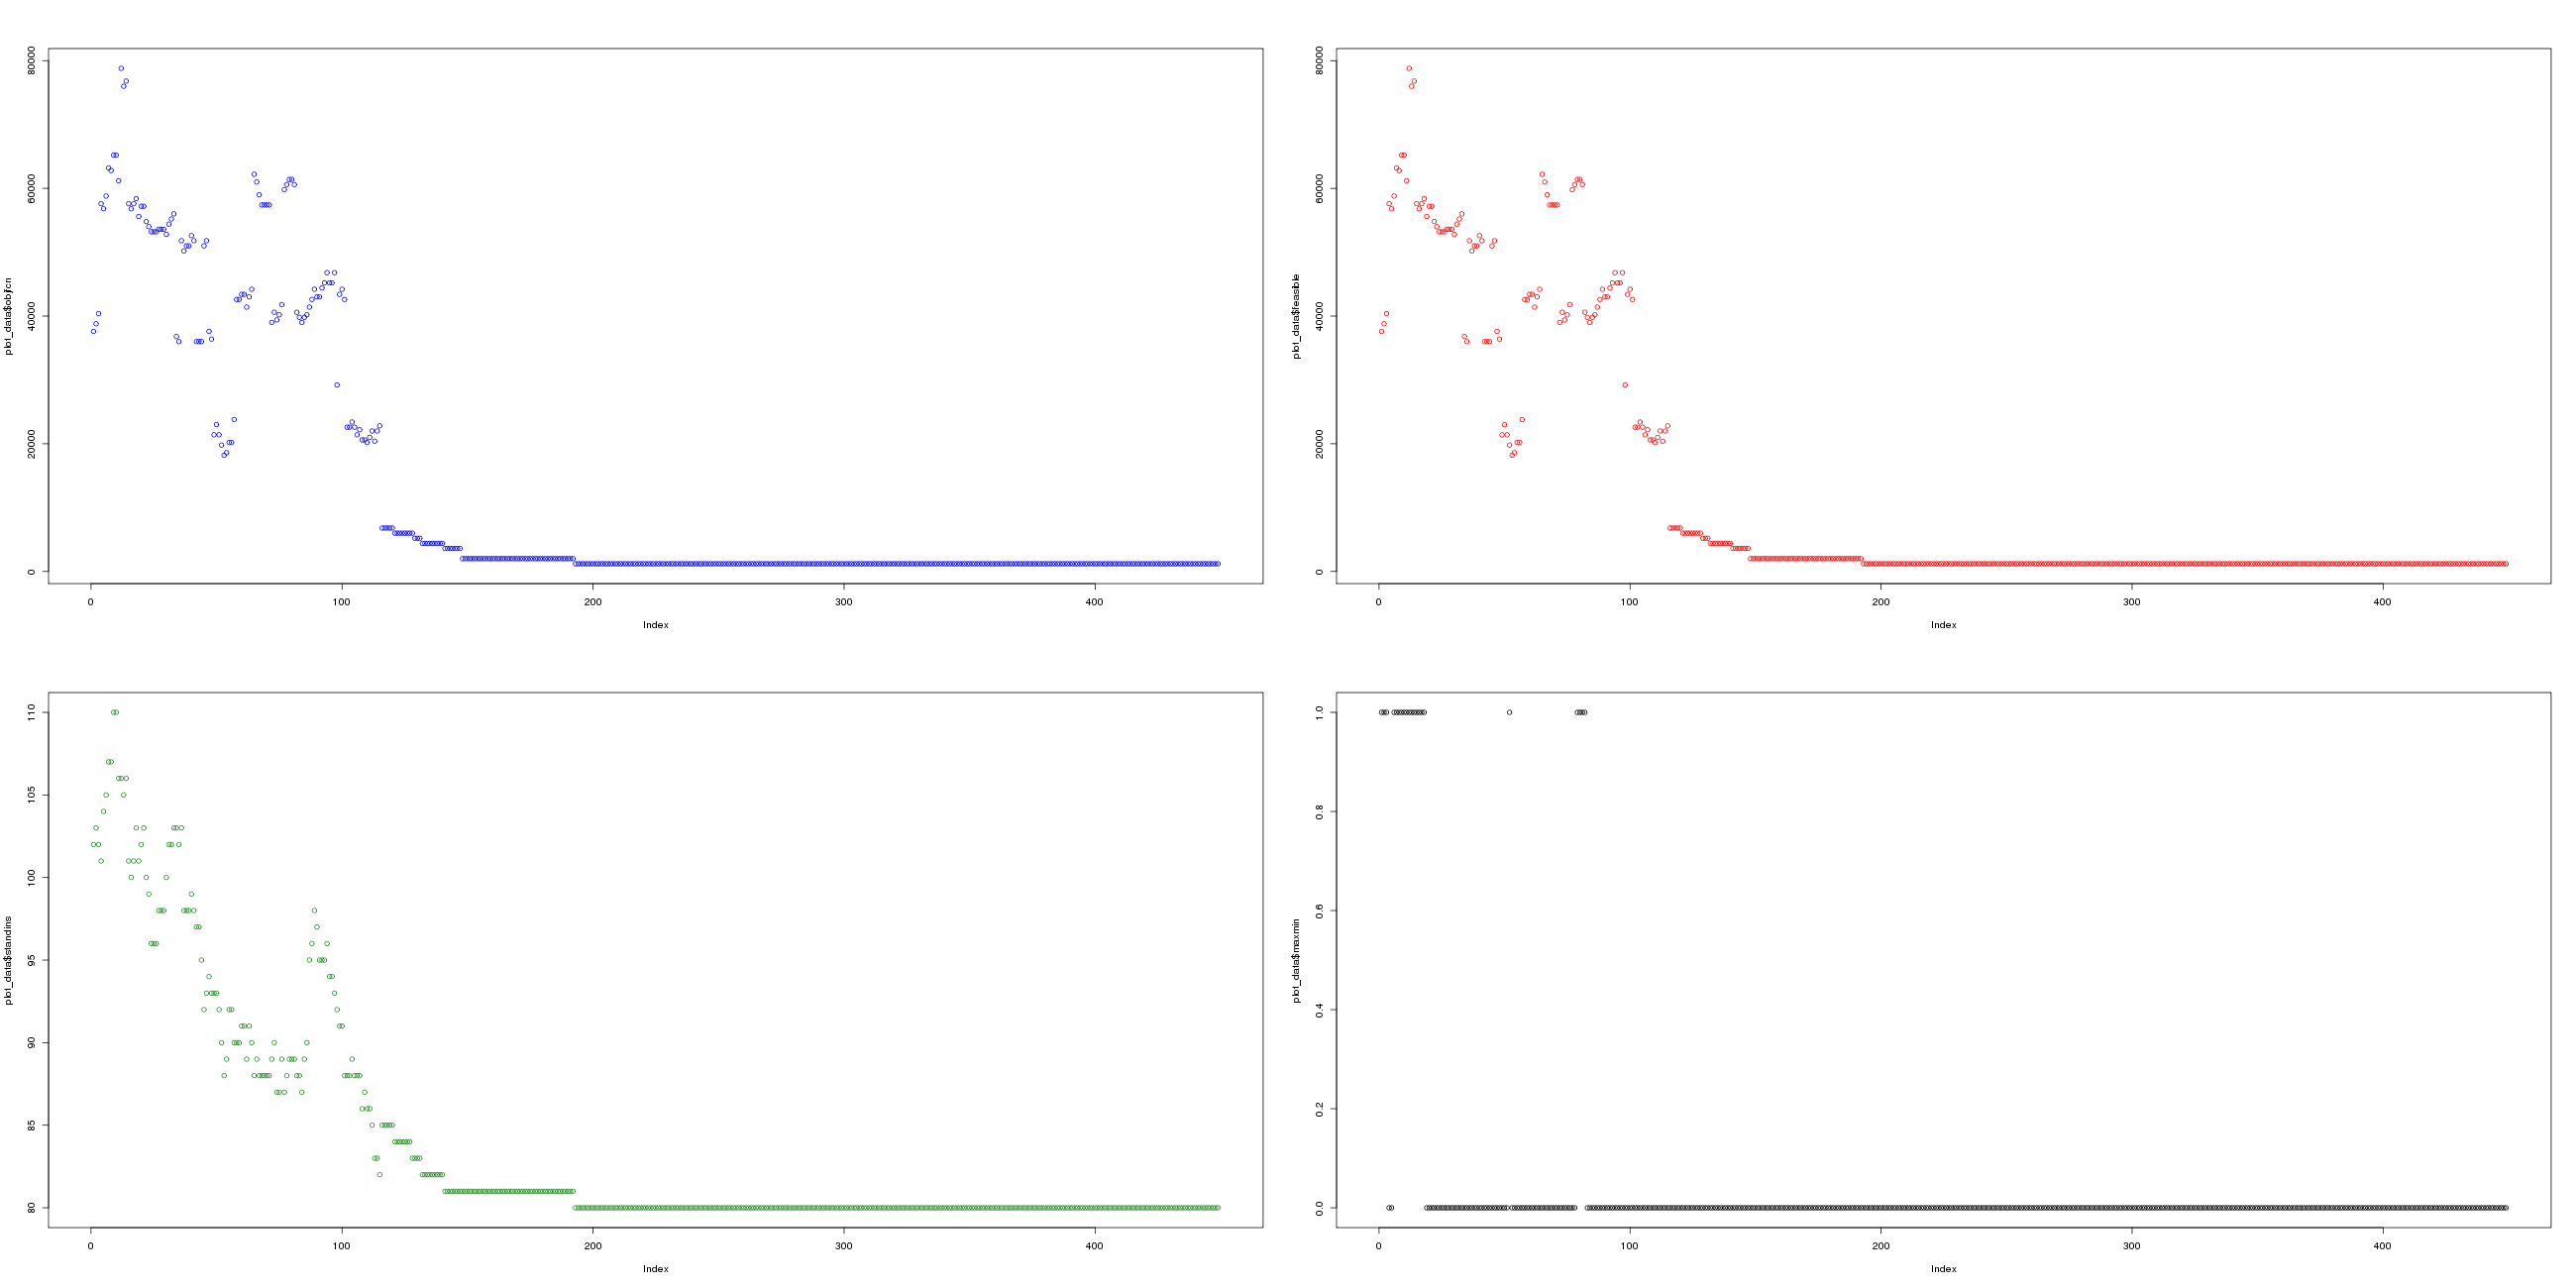
\includegraphics[scale = 0.3, width = 15cm]{Rplot}
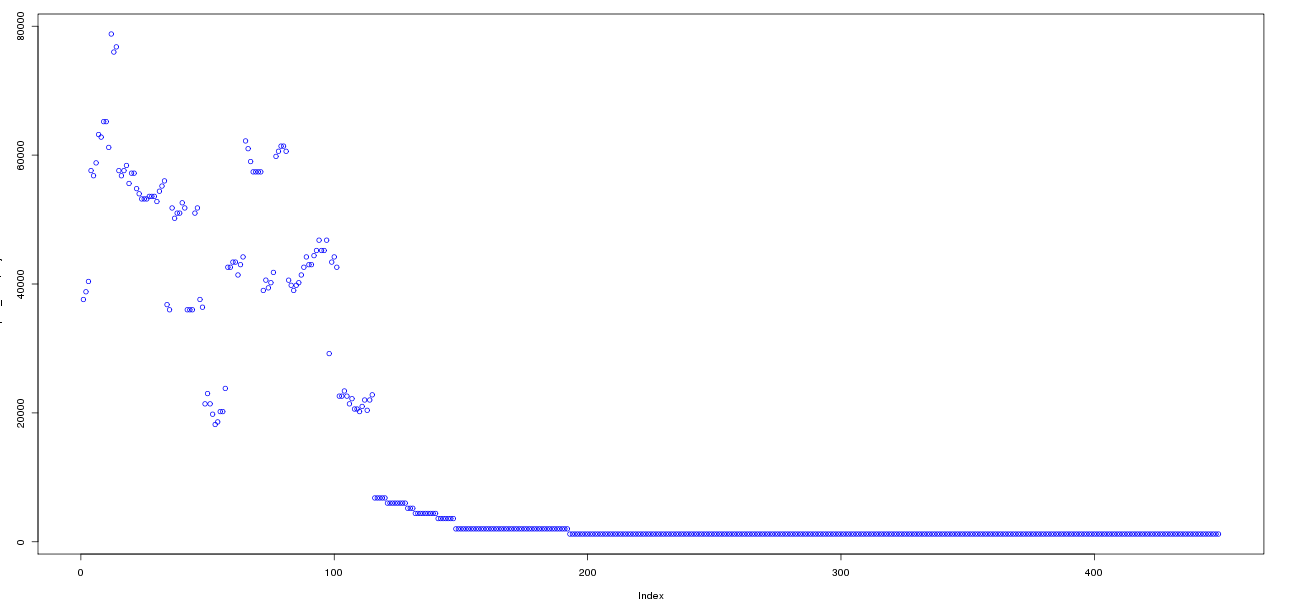
\includegraphics[scale = 0.3, width = 15cm]{1Plot}
\subsection{Task distribution approach}

Some parameter tuning was done in order to find the optimal settings for the algoritm, particularly for the weekend objective function weights described in Section \ref{section:tasks_cost}. The tuning landed in the following parameters
 
Number of iterations, first phase.
Number of iterations, second phase.
$T_0$, $\alpha$


\section{Discussion}
Text


\subsection{Weekly scheduling approach}
Table \ref{pros_cons_weekly_scheduling} lists pros and cons with the implemented weekly scheduling approach. Some pros and cons were considered before the heuristic was chosen. Mainly the con concerning the exponential growth was taken into consideration as an estimation of the upper limit of the problem size was done. Also, the pro regarding the same amount of week blocks was taken into consideration, as the heuristic was thought of having firstly a block construction phase and secondly an assignment phase. 

\begin{table}[!h]
\caption{Pros and cons with the implemented weekly scheduling approach}
\label{pros_cons_weekly_scheduling}
\begin{tabularx}{\linewidth}{>{\parskip1ex}X@{\kern4\tabcolsep}>{\parskip1ex}X}
\toprule
\hfil\bfseries Pros
&
\hfil\bfseries Cons
\\\cmidrule(r{3\tabcolsep}){1-1}\cmidrule(l{-\tabcolsep}){2-2}

%% PROS, seperated by empty line or \par
The same amount of week block appearances will exist for five and ten weeks.\par
Quick iterations when destroying and repairing.\par

&

%% CONS, seperated by empty line or \par
Weekends needs to be assigned in a more systematically way in order to achieve reasonable results regarding lowest amount of stand-ins through the days.\par
The amount of unique block appearances grows exponentially in case more task types are added, such as meetings.\par
The solution time can vary considerably as several random generators have been used.\par
A great deal of costs are needed (some correlated), where each of them affects the solution procedure.

\\\bottomrule
\end{tabularx}
\end{table}

 Weekends, solution time and costs are no major issues as they can be avoided by a few smarter implementations. For instance, weekends can be improved by assigning values when each worker is available on a day and from those numbers create an even distribution of possible stand-ins and therefore increase the lowest value of stand-ins through the days. This shall implicitly decrease the solution time as less iterations will be required. However, to always be able to create a pool of week appearances regardless of problem size can easily become a major issue. Just by adding meetings and the assignment of Library on Wheels tasks to the problem makes it grow considerably.
 

\subsection{Task distribution approach}
Text
\inputencoding{\enc}

\chapter{Further development}\label{chap:further}
\inputencoding{\enc}
For both of the heuristics the first step is to generalize the problem to ten weeks instead of five. In doing so, the heuristics will have the same time span as the AMPL implementation. Furthermore, if meetings are implemented and five-week separated work weeks look alike the heuristics will solve the same problem as the AMPL implementation. 

By looking at the results from the heuristics it deems possible to solve the complete problem by spending more time implementing. However, regardless if such results were reached it would only work for this specific library. A general solver would not be a feature that could be implemented. The reason is due to the uniqueness of requirements in the library. In case they were similar someone would, most likely, already have created a general solver for libraries or any other service institution.
\inputencoding{\enc}

\chapter{Conclusion}\label{chap:concl}
\inputencoding{\enc}
In this thesis work, a mathematical model for the given staff scheduling problem at the Library of Norrköping was developed. The model was run on the commercial optimization solver CPLEX, which generated an optimal schedule with three librarian stand-ins and zero assistant stand-ins at the worst day. This is better than the current schedule at the library, where only one staff member was assigned as stand-in on the worst day.

When developing the two heuristics for solving the problem, the conclusion was reached that the weekend distribution is essential for the stand-in distribution in the final schedule. The heuristic which focused on weekend scheduling separate from the rest of the problem thus performed better. 

Although good results were obtained both by using the AMPL model and the second heuristic, there is room for further development in the modeling of the problem. One of the things which could be done in a more robust way is the modeling of exceptions and preferences among the staff members. In the current model, these are simply modeled as hard constraints. If these could be modeled in a more general way or in separation from the core problem, the model would not be so sensitive to changes in exceptions or staff preferences.

Several components of the model could be simplified. For example, the library on wheels could be modeled separately from the rest of the problem. Another suggestion is to simplify every other week staff memebers' schedules so that the person gets two five week schedules instead. Also, a more general way of describing meetings would simplify their distribution. One way of doing this could be to produce schedules which are not entirely feasible according to the problem description, but which can be used as a basis for manual scheduling.

Regarding the implementations, there are several components missing in order for the heuristics to fully correspond to the mathematical model. Although these features are not crucial, they could be implemented in order to make the heuristics correspond to the full problem. Furthermore, a more systematic framework for testing and evaluating the heuristics could be developed in order to be able to measure results which are more comparable.



% % OLD CONCLUSION % %
%In this thesis work, a mathematical model for the given staff scheduling problem at the Library of Norrköping was developed. The model was run on the commercial optimization solver CPLEX, which generated an optimal schedule with three librarian stand-ins and zero assistant stand-ins at the worst day. This is better than the current schedule at the library, where only one staff member was assigned as stand-in on the worst day.

%When developing the two heuristics for solving the problem, the conclusion was reached that the weekend distribution is essential for the stand-in distribution in the final schedule. The heuristic which focused on weekend scheduling separate from the rest of the problem thus performed better. It was also concluded that the problem is not very difficult to solve, however it is challenging to model. In order to find a more robust scheduler for the problem, which can adapt to changes in the work force, a better model must be developed.


% To CLaes: is it possible to focus on weekends using your implementation?
\inputencoding{\enc}


%##########################################################
% -------------------END CHAPTERS -------------------------
%##########################################################

\bibliography{Chapters/References}


%%% .................. appendix ...................................
\appendix
\chapter{Problem definitions} \label{definitions}
\section{Sets}
\itab{I} \tab{Set of workers}\\
\itab{I\_lib} \tab{Set of librarians (I\_lib $\subseteq$ I)} \\
\itab{I\_ass}	 \tab{Set of assistants (I\_ass $\subseteq$ I)}	\\
\itab{W}                 \tab{Set of weeks}                                               \\
\itab{D}                 \tab{Set of days in a week}                                      \\
\itab{$S_d$}           \tab{Set of shifts day \textit{d}}                                        \\
\itab{$J_d$}            \tab{Set of task types day \textit{d}}                                    \\
\itab{I\_LOW}	 \tab{Set of librarians available to work in library on wheels}	\\
\itab{I\_free\_day}	 \tab{Set of workers that shall be assigned a free weekday per week}	\\
\itab{I\_odd\_even}	 \tab{Set of all workers with odd or even weeks}	\\
\itab{I\_weekend\_avail}	 \tab{Set of workers available for weekend work}	\\ 
\newpage
\section{Variables} \label{variabs}
\begin{align}
    x_{iwdsj}&=
    \begin{cases}
      1, & \text{if worker \textit{i} is assigned in week \textit{w}, day \textit{d}, shift \textit{s} to a task \textit{j}}\\
      0, & \text{otherwise}
    \end{cases}
    \\
    H_{iwh}&=
    \begin{cases}
      1, & \text{if worker \textit{i} works weekend h in week \textit{w}}\\
      0, & \text{otherwise}
    \end{cases}
	\\
	r_{iw}&=
	\begin{cases}
		1, & \text{if worker \textit{i} has its scheduled rotated \textit{w-1 steps}}\\
		0, & \text{otherwise}
	\end{cases}
	\\
	lib_{iwd}&=
	\begin{cases}
	  1, & \text{if librarian \textit{i} is a stand-in week \textit{w} day \textit{d}} \\
	  0, & \text{otherwise}
	\end{cases}
	\\
	ass_{iwd}&=
	\begin{cases}
 		1, & \text{if assistant \textit{i} is a stand-in week \textit{w} day \textit{d}} \\
 		0, & \text{otherwise}
	\end{cases}
	\\
	y_{iwds}&=
	\begin{cases}
 		1, & \text{if worker \textit{i} is working \textit{w} day \textit{d} regardless of task type} \\
 		0, & \text{otherwise}
	\end{cases}
	\\
	hb_{iw}&=
	\begin{cases}
 		1, & \text{if assistant \textit{i} is a stand-in week \textit{w} day \textit{d}} \\
 		0, & \text{otherwise}
	\end{cases}
	\\
	friday\_evening_{iw}&=
	\begin{cases}
 		1, & \text{if assistant \textit{i} is a stand-in week \textit{w} day \textit{d}} \\
 		0, & \text{otherwise}
	\end{cases}	
	\\
	lib\_min&= \text{lowest number of stand-in librarians found (integer)} \\
	ass\_min&= \text{lowest number of stand-in assistants found (integer)}
\end{align}
\newpage
\section{Parameters} \label{params}
\begin{align}
	N1l&= \text{a value to prioritize the amount of stand-in librarians}
	\\
	N1a&= \text{a value to prioritize the amount of stand-in assistants}
	\\
	N2&= \text{a value to prioritize similar weeks}
	\\
	avail\_day_{iwd}&=
	\begin{cases}
		1, & \text{if worker \textit{i} is available for work week \textit{w}, day \textit{d}} \\
		0, & \text{otherwise}
	\end{cases}
	\\
	task\_demand_{dsj}&= \text{number of workers required day \textit{d}, shift \textit{s} for task type \textit{j}}
	\\
	qualavail_{iwdsj}&=
	\begin{cases}
		1, & \text{if worker \textit{i} is qualified and available week \textit{w}, day \textit{d}, shift \textit{s} for task type \textit{j}} \\
		0, & \text{otherwise}
	\end{cases}
	\\
	LOW\_demand_{wds}&= \text{number of workers required day \textit{d}, shift \textit{s} at the library on wheels}
\end{align}

% % %New chapter
\chapter{Flow charts} \label{appendix:flow_charts}

% Define block styles
\tikzstyle{decision} = [diamond, draw, fill=red!30,
    text width=3.5em, text badly centered, node distance=3cm, inner sep=0.1pt]
\tikzstyle{block} = [rectangle, draw, fill=blue!30,
    text width=5em, text centered, rounded corners, minimum height=4em]
\tikzstyle{line} = [draw, -latex']
\tikzstyle{cloud} = [draw, ellipse,fill=red!20, node distance=3cm,
    minimum height=2em]


\section{Weekly scheduling approach}
% % FLOW CHART
\begin{figure}[!h]
  \caption{A flow chart of the implemented heuristic with weekly scheduling}
  \centering
	\scalebox{0.7}{ \label{flow_chart}
		\begin{tikzpicture}[node distance = 2cm, auto]
		    % Place nodes
			\node [block] (blocks) {Create all blocks};
			\node [block,below of= blocks] (workers) {Create all workers};
			\node [block,below of= workers] (sort) {Sort blocks to workers};
			\node [block,below of= sort] (assign_rot) {Assign rotations};
			\node [block,below of= assign_rot] (assign_low) {Assign LoW schedule};
			\node [block,below of= assign_low] (init_sol) {Create initial solution};
			\node [decision, right of = init_sol, node distance= 4cm] (feasible) {Is solution feasible?};
			\node [block,above of= feasible, node distance = 3cm] (repair) {Repair workers};
			\node [block,above of= repair, node distance = 2cm] (destroy) {Destroy workers};
			
			
			\node [block,below of= feasible, node distance = 6cm] (print) {Print solution to file};
			\node[decision,right of= feasible, node distance=3.5cm] (close) {Close enough?};
			\node[block,below of= close, node distance = 3cm] (final) {Enter final phase};
			\node[decision, right of= final, node distance = 4cm] (solved) {Solved in given number of iterations?};
			\node[block,right of= assign_low, node distance = 11.5cm] (failed) {Failed iteration, run again};
			
			
			%Invisible node, useful later
			\node[right of= sort, node distance=5.5cm,scale=0.01](invLNS){};
			\node[above of= blocks, node distance=1.3cm,scale=0.01](inv){};
			
			\node[above of= invLNS, node distance = 0.7cm] (text) {LNS};
			
		    % Draw edges
		    \path [line] (inv) -- (blocks);
		    \path [line] (blocks) -- (workers);
		    \path [line] (workers) -- (sort);
		    \path [line] (sort) -- (assign_rot);
		    \path [line] (assign_rot) -- (assign_low);
		    \path [line] (assign_low) -- (init_sol);
		    \path [line] (init_sol) |- (feasible);
		    \path [line] (destroy) -- (repair);
		    \path [line] (repair) -- (feasible);
		    \path [line] (feasible) -- node[right]{yes}(print);
		    \path [line] (feasible) -- node[above]{no}(close);
		    \path [line] (close) |- node[right]{no}(destroy);
		    \path [line] (close) -- node[right]{yes}(final);
		    \path [line] (final) -- (solved);
		    \path [line] (solved) |- node[right]{yes}(print);
		    \path [line] (solved) -- node[right]{no}(failed);
		    \path [line] (failed) |- (blocks);
%			\path[-,draw] (feasible) -| node[right]{no} (inv.north);
%		    \path[line]{} (inv.north) |- node{} (destroy);
			\draw [color=gray!70,thick](2.3,-3.5) rectangle(6,-12);
		\end{tikzpicture}
		}
\end{figure}


\section{Task distribution approach}

\begin{figure}[h]
\centering
\caption{Algorithm for distributing weekends.}
\label{fig:weekend_alg}
\scalebox{0.6}{
\begin{tikzpicture}[node distance = 2cm, auto]
    % Place nodes
    %Right row
    \node [scale=0.01,node distance=0cm] (invinit) {};
    \node [block, below of=invinit] (distribute) {Distribute all weekends randomly};
    \node [decision, below of=distribute, node distance=2.5cm] (evaluate) {Solution feasible?};
    \node [block, left of=distribute, node distance=4cm] (redistribute) {Remove all weekends};
     \node [block, below of=evaluate, node distance=3.5cm] (setobjf) {Set weekend obj fun value};
     \node [block, below of=setobjf, node distance=3cm] (save) {Save temp solution};
     \node [block, below of=save, node distance=3cm] (dr) {Destroy and repair solution};
     \node [decision, below of=dr] (evaluate2) {Solution feasible?};
     \node [block, right of=dr, node distance=3cm] (reload) {Reload temp solution};
     
     %Middle row
     \node [block, left of=evaluate2, node distance=5cm] (setobjf2) {Set weekend obj fun value};
     \node [decision, above of=setobjf2, node distance=2.5cm] (compare) {Better than saved?};
     \node [decision, above of=compare, node distance=2.5cm] (SA) {Accept anyway?};
     \node [decision, left of=SA, node distance=4cm] (best) {Best solution?};
     \node  [block, above of=SA, node distance =2.5cm] (reloadsaved) {Reload saved solution}; 
     \node [block, above of=best, minimum height=3em, node distance = 2cm] (savebest) {Save solution as best};
     \node [decision, above of=reloadsaved, node distance=2cm] (done) {Iteration \textgreater max?};
     \node[above of=savebest, left of=savebest, node distance=2.5cm, scale=0.1](inv){};
     
     %Bottom nodes
     \node [decision, below of=best, node distance=10cm] (isbest) {Current better than best?};
     \node [block, right of=isbest, minimum height=3em, node distance=3cm] (reload2) {Reload best};
      \node [block, below of=reload2, minimum height=3em, node distance=2.5cm] (finished) {Search finished!};

    % Draw edges
    \path [line] (invinit) -- (distribute);
    \path [line] (distribute) -- (evaluate);
    \path [line] (evaluate) -| node {no} (redistribute);
    \path [line] (redistribute) |- (distribute);
    \path [line] (evaluate) -- node {yes}(setobjf);
    \path [line] (setobjf) -- (save);
    \path [line] (save) -- (dr);
    \path [line] (dr) -- (evaluate2);
    \path [line] (evaluate2) -| node {no} (reload);
    \path [line] (reload) -- (dr);
    \path [line] (evaluate2) -- node {yes} (setobjf2);
    \path [line] (setobjf2) -- (compare);
    \path [line] (compare) -| node {yes} (best);
    \path [line] (compare) -- node {no} (SA);
    \path [line] (SA) -- node {yes} (best);
    \path [line] (SA) -- node {no} (reloadsaved);
    \path [line] (reloadsaved) -- (done);
    \path [line] (best) -- node {yes} (savebest);
    \path [line] (best) -- node {no} (done);
    \path [line] (savebest) -- (done);
    \path [line] (done) -- node {no}(save);
    \path [-,draw] (done) -- node {yes}(inv);
    \path [line] (inv) |- (isbest);
    \path [line] (isbest) -- node {no} (reload2);
    \path [line] (isbest) -- node {yes} (finished);
    \path [line] (reload2) -- (finished);
   
    %Feasiblity loop
    \node at (-2,-19) [above=4mm, right=2mm] {\textsc{destroy and repair loop}};
    \draw [color=gray!70,thick](-2,-19) rectangle (5,-12);
    %Weekend loop
    \node at (-10.5,-19.5) [above=4mm, right=2mm] {\textsc{weekend distribution loop}};
    \draw [color=gray!70,thick](-10.5,-19.5) rectangle (5,-6);
    %SA componenet
    \node at (-7.5,-13.5) [above=4mm, right=2mm] {\textsc{SA}};
    \draw [color=gray!70,thick](-7.5,-13.5) rectangle (-3,-10.5);
\end{tikzpicture}
}
\end{figure}


\begin{figure}[!h]
\centering
\caption{Algorithm for distributing weekday tasks.}
\label{fig:weekday_alg}
\scalebox{0.8}{
\begin{tikzpicture}[node distance = 2cm , auto, every node/.style={scale=0.8}]
    %Right column
    \node [scale=0.01,node distance=0cm] (invinit) {};
    \node [block, below of=invinit] (distribute) {Try distribute all tasks};
    \node [block, below of=distribute] (workercost) {Set worker obj fun};
    \node [decision, below of=workercost, node distance=2.5cm] (evaluatewc) {Worker cost = 0?};
    \node [decision, below of=evaluatewc, node distance=3cm] (evaluatetasks) {All tasks distributed?};
    \node [decision, below of=evaluatetasks, node distance=3cm] (feasible) {Solution feasible?};
    \node [block, below of=feasible, node distance=2.5cm] (destamount) {Set destroy amount};
    \node [block, below of=destamount] (dr) {Destroy and repair solution};

    %Middle column
     \node [block, left of=evaluatetasks, node distance = 4cm] (taskcost) {Set weekday costs};
    \node [decision, above of=taskcost, node distance=2cm] (best) {Best solution?};
    \node [block, above of=best, minimum height=3em, node distance = 2cm] (savebest) {Save solution as best};
    
    %Left column
    \node [decision, left of=savebest, node distance=4cm] (done) {Iteration \textgreater max?};
    \node [block, above of=done, node distance=3.5cm] (remove) {Remove all tasks};
    
    %Get solution
    \node [decision, below of=done, node distance=15cm] (isbest) {Current better than best?};
    \node [block, right of=isbest, minimum height=3em, node distance=3cm] (reload2) {Reload best};
    \node [block, below of=reload2, minimum height=3em, node distance=2.5cm] (finished) {Search finished!};
    
	%Invisible nodes
    \node [right of=evaluatewc, scale=0.1,node distance=2cm] (inv) {};
    \node [right of=dr, scale=0.1,node distance=4cm] (inv2) {};
    \node [right of=workercost, scale=0.1,node distance=4cm] (inv3) {};
    \node[left of=isbest, node distance=4cm, scale=0.1](inv4){};
    
 
	%Draw edges
	\path [line] (invinit) -- (distribute);
    \path [line] (distribute) -- (workercost);
    \path [line] (workercost) -- (evaluatewc);
    \path [line] (evaluatewc) -- node [anchor=east]{yes} (evaluatetasks);    
    \path [-,draw] (evaluatewc) -- node [anchor=south]{no} (inv);    
    \path [line] (evaluatetasks) -- node [anchor=south]{yes} (taskcost);
    \path [line] (evaluatetasks) -- node [anchor=east]{no} (feasible);
    \path [line] (destamount) -- (dr);
    \path [-,draw] (dr) -- (inv2);
    \path [-,draw] (inv2) -- (inv3);
    \path [line] (inv3) -- (workercost);
     %To middle row   
	\path [line] (inv) |- (feasible);
    \path [line] (feasible) -- node [anchor=east]{yes} (destamount);
    \path [line] (feasible) -| node [anchor=east]{no} (done);
    %Middle row
    \path [line] (done) -- node [anchor=east]{no}(remove);    
    \path [line] (best) -- node [anchor=east]{yes}(savebest);
    \path [line] (savebest) -- (done);
    \path [line] (best) -- node [anchor=east]{no}(done);
    \path [line] (taskcost) -- (best);
    \path [line] (remove) -- (distribute);
    \path [-,draw] (done) -| node [anchor=east] {yes} (inv4);
    \path [line] (inv4) -- (isbest);
    \path [line] (isbest) -- node [anchor=south]{no} (reload2);
    \path [line] (isbest) -- node [anchor=east]{yes} (finished);
    \path [line] (reload2) -- (finished);

    %Feasiblity loop
    \node at (-2,-15) [above=4mm, right=2mm] {\textsc{destroy and repair loop}};
    \draw [color=gray!70,thick](-2,-15) rectangle (4,-2.5);
    %Weekend loop
    \node at (-8,-15) [above=4mm, right=2mm] {\textsc{weeday task distribution loop}};
    \draw [color=gray!70,thick](-8,-15) rectangle (4,-0.5);

\end{tikzpicture}
}
\end{figure}


\chapter{Weekblock table} \label{appendix:weekblock}
\begin{table}[!h]
\centering
\caption{Number of assignable unique blocks for the workers based on their availability and qualification.}
\label{blocks_available_per_worker}
\scalebox{0.75}{
	\begin{tabular}{|c|ccc|}
	\hline
	Worker & Weekend & Weekrest & Weekday \\ \hline
	1      & 532     & 347      & 1580    \\ \hline
	2      & 1580    & 1580     & 1580    \\ \hline
	3      & 1063    & 347      & 1580    \\ \hline
	4      & 557     & 165      & 779     \\ \hline
	5      & 261     & 130      & 531     \\ \hline
	6      & 532     & 130      & 1580    \\ \hline
	7      & 261     & 130      & 531     \\ \hline
	8      & 261     & 29       & 531     \\ \hline
	9      & 115     & 12       & 247     \\ \hline
	10     & 532     & 130      & 1580    \\ \hline
	11     & 9       & 8        & 8       \\ \hline
	12     & 1063    & 347      & 1580    \\ \hline
	13     & 771     & 92       & 1190    \\ \hline
	14     & 265     & 29       & 489     \\ \hline
	15     & 51      & 18       & 120     \\ \hline
	16     & 495     & 130      & 843     \\ \hline
	17     & 237     & 69       & 267     \\ \hline
	18     & 532     & 279      & 1580    \\ \hline
	19     & 495     & 47       & 843     \\ \hline
	20     & 532     & 130      & 1580    \\ \hline
	21     & 227     & 227      & 227     \\ \hline
	22     & 2       & 1        & 1       \\ \hline
	23     & 3       & 2        & 2       \\ \hline
	24     & 11      & 5        & 47      \\ \hline
	25     & 1063    & 279      & 1580    \\ \hline
	26     & 5       & 4        & 4       \\ \hline
	27     & 213     & 106      & 425     \\ \hline
	28     & 2       & 2        & 2       \\ \hline
	29     & 426     & 106      & 1281    \\ \hline
	30     & 127     & 126      & 455     \\ \hline
	31     & 495     & 130      & 843     \\ \hline
	32     & 261     & 29       & 531     \\ \hline
	33     & 72      & 45       & 306     \\ \hline
	34     & 425     & 425      & 425     \\ \hline
	35     & 91      & 20       & 221     \\ \hline
	36     & 55      & 27       & 101     \\ \hline
	37     & 1063    & 347      & 1580    \\ \hline
	38     & 3       & 1        & 1       \\ \hline
	39     & 2       & 1        & 1       \\ \hline
	\end{tabular}
	}
\end{table}

% this is the copyright page, I did not touch it much.

\cleardoublepage

\thispagestyle{plain}

\begin{picture}(20,20)(0,0)
% \put(0,10){\includegraphics[width=3.5cm]{epresslogo}}
\put(280,0){
\includegraphics[width=2.5cm]{univlogo.eps}}
\end{picture}
 
\null
\vspace{0cm} 

Copyright
\medskip

The publishers will keep this document online on the Internet - or its possible replacement - for a period of 25 years from the date of publication barring exceptional circumstances.
The online availability of the document implies a permanent permission for anyone to read, to download, to print out single copies for your own use and to use it unchanged for any non-commercial research and educational purpose. Subsequent transfers of copyright cannot revoke this permission. All other uses of the document are conditional on the consent of the copyright owner. The publisher has taken technical and administrative measures to assure authenticity, security and accessibility.
According to intellectual property law the author has the right to be mentioned when his/her work is accessed as described above and to be protected against infringement.
For additional information about the Linköping University Electronic Press and its procedures for publication and for assurance of document integrity, please refer to its WWW home page: http://www.ep.liu.se/
\bigskip

Upphovsr\"att
\medskip

Detta dokument hålls tillgängligt på Internet - eller dess framtida ersättare - under 25 år från publiceringsdatum under förutsättning att inga extraordi\-nära omständigheter uppstår.
Tillgång till dokumentet innebär tillstånd för var och en att läsa, ladda ner, skriva ut enstaka kopior för enskilt bruk och att använda det oförändrat för ickekommersiell forskning och för undervisning. Överföring av upphovsrätten vid en senare tidpunkt kan inte upphäva detta tillstånd. All annan användning av dokumentet kräver upphovsmannens medgivande. För att garantera äktheten, säkerheten och tillgängligheten finns det lösningar av teknisk och administrativ art.
Upphovsmannens ideella rätt innefattar rätt att bli nämnd som upphovsman i den omfattning som god sed kräver vid användning av dokumentet på ovan beskrivna sätt samt skydd mot att dokumentet ändras eller presenteras i sådan form eller i sådant sammanhang som är kränkande för upphovsmannens litterära eller konstnärliga anseende eller egenart.
För ytterligare information om Linköping University Electronic Press se förlagets hemsida http://www.ep.liu.se/

\medskip

\copyright\phantom{.} \putshortdate, \putauthor




%----------------END OF DOCUMENT----------------------------------------------
%----------------END OF DOCUMENT----------------------------------------------

\end{document}
 
